%%
%% This is file `sample-acmsmall.tex',
%% generated with the docstrip utility.
%%
%\documentclass[acmsmall,screen,review]{acmart}
\documentclass[acmsmallw,review]{acmart}
%%
%% \BibTeX command to typeset BibTeX logo in the docs
\AtBeginDocument{%
  \providecommand\BibTeX{{%
    \normalfont B\kern-0.5em{\scshape i\kern-0.25em b}\kern-0.8em\TeX}}}

\setcopyright{acmcopyright}
\copyrightyear{2026}
\acmYear{2026}
\acmDOI{XXXXXXX.XXXXXXX}

%% These commands are specific to PACMPL (for OOPSLA Round 2)
\acmJournal{PACMPL}
\acmVolume{1}
\acmNumber{OOPSLA2}
\acmArticle{1}
\acmMonth{1}


%% Packages
\usepackage{booktabs} % For formal tables
\usepackage{stmaryrd}
\usepackage{adjustbox}
\usepackage{subcaption}

\usepackage{algorithm}
\usepackage{algpseudocode}

% TikZ and Quantikz
\usepackage{tikz}
\usetikzlibrary{quantikz2}
\usetikzlibrary{shapes.geometric, arrows}

% Comment commands
\newcommand{\showcomment}[1]{#1}
%\renewcommand{\showcomment}[1]{} % Set to empty to hide comments


%\newcommand{\yfc}[1]{\showcomment{\textcolor{purple}{\textbf{YFC:} #1}}}
%\newcommand{\bw}[1]{\showcomment{\textcolor{green}{\textbf{BW:} #1}}}
%\newcommand{\cy}[1]{\showcomment{\textcolor{blue}{\textbf{CY:} #1}}}
%\newcommand{\rmark}[1]{\textcolor{red}{#1}}

% Temporarily hide all comments:
\newcommand{\yfc}[1]{}
\newcommand{\bw}[1]{}
\newcommand{\cy}[1]{}

\citestyle{acmauthoryear}

\begin{document}

\title{Formal Verification of Fault-Tolerant Flagged Syndrome Extraction Protocols}

\author{Bo-Ruei Wu}
\affiliation{%
  \institution{Academia Sinica}
  \city{Taipei}
  \country{Taiwan}
}

\author{Yu-Fang Chen}
\affiliation{%
  \institution{Academia Sinica}
  \city{Taipei}
  \country{Taiwan}
}

\author{Ching-Yi Lai}
\affiliation{%
  \institution{National Yang Ming Chiao Tung University}
  \city{Hsinchu}
  \country{Taiwan}
}

\begin{abstract}
Fault-tolerant syndrome extraction protocols using flag qubits can reduce the number of required ancilla qubits or circuit rounds, making them attractive for near-term fault-tolerant quantum computing architectures. However, the design and validation of such circuits typically rely on intricate manual analysis of error propagation patterns. Ensuring that all possible fault combinations are properly accounted for can be challenging. Subtle issues in gate ordering, ancilla interactions, or measurement scheduling may lead to unintended error propagation, resulting in correlated data errors and, in the worst case, logical failures.

In this work, we propose a SAT-based formal verification framework for \emph{flagged syndrome extraction protocols}. We focus on a central correctness property: for any set of up to $t = \lfloor (d-1)/2 \rfloor$ circuit-level faults, the resulting data errors must either be non-degenerate or yield distinguishable syndrome and flag outcomes. We encode Pauli fault propagation, measurement behavior, and bounded-fault constraints as Boolean formulas, and verify correctness by proving the unsatisfiability of configurations that violate this property.
 
Using our framework, we analyze several representative flagged circuits and identify design flaws that violate the specified correctness property. Our results demonstrate that SAT-based formal verification provides a rigorous and systematic approach to validating fault-tolerant quantum circuit constructions.
\end{abstract}

%\cy{don't say Liou and Bhatnagar; cite their papers in the manuscript}

\begin{CCSXML}
<ccs2012>
   <concept>
       <concept_id>10010583.10010786.10010813</concept_id>
       <concept_desc>Hardware~Quantum error correction and fault tolerance</concept_desc>
       <concept_significance>500</concept_significance>
   </concept>
   <concept>
       <concept_id>10003752.10003790.10003794</concept_id>
       <concept_desc>Theory of computation~Automated reasoning</concept_desc>
       <concept_significance>500</concept_significance>
   </concept>
 </ccs2012>
\end{CCSXML}

\ccsdesc[500]{Hardware~Quantum error correction and fault tolerance}
\ccsdesc[500]{Theory of computation~Automated reasoning}

\keywords{Fault tolerant quantum computing, Verification, SAT}

\maketitle

\bw{change ST solver}
\section{Introduction}

Quantum computing promises asymptotic advantages over classical computation. However, realizing these advantages requires protection against noise. Physical qubits are subject to frequent faults from decoherence and imperfect gates. 
Quantum error-correcting codes (QECCs) address this challenge by encoding logical information into multiple physical qubits. A code of distance $d$ can theoretically correct up to $t = \lfloor (d-1)/2 \rfloor$ errors. However, this guarantee relies on a crucial assumption: that the error-correction circuitry itself operates reliably.

To reason about reliability more precisely, we distinguish between \emph{faults} and \emph{errors}.
A fault is a circuit-level malfunction, such as a faulty gate or measurement operation. Under the Pauli circuit-level noise model considered in this work, each fault introduces a Pauli error that propagates through the circuit. An error denotes the resulting Pauli operator acting on the data qubits. A protocol is fault-tolerant if, for any set of at most 
$t$ faults, the induced data error remains correctable for the underlying quantum code.
In practice, faults may occur during the error-correction procedure. A single internal fault can propagate through the circuit, producing correlated data errors that exceed the code's correction capability and lead to logical failure.

To address the challenge of fault-tolerant error correction (FTEC), schemes such as those proposed by Shor \cite{Shor96}, Steane \cite{Steane97}, and Knill \cite{Knill05} were developed. While these approaches are conceptually elegant, they require substantial ancillary resources and multiple rounds of verification, leading to considerable overhead for near-term architectures. 

Flagged syndrome extraction protocols offer a resource-efficient alternative. Instead of using encoded states, these protocols instrument the circuit with unencoded \emph{flag qubits}. These flags act as runtime monitors: they signal when a dangerous internal fault has occurred. The control logic then uses this signal to adapt the recovery strategy.

Flagged syndrome extraction protocols were pioneered by Chao and Reichardt~\cite{Chao18} for a family of distance-3 codes. This approach was subsequently generalized to codes of arbitrary distance by Chamberland and Beverland~\cite{Chamberland18}. More recent research has focused on optimizing these protocols to reduce resource overhead: Reichardt~\cite{reichardt2021fault}, Liou and Lai~\cite{LL23,Liou25}, and Du et al.~\cite{Du24} introduced parallelization and flag-sharing techniques to minimize circuit depth and qubit count. Other approaches, such as low-depth adaptive protocols~\cite{low-depth}, further optimize execution by dynamically selecting specific stabilizers to measure based on intermediate outcomes.

However, designing these protocols is essentially a complex synthesis problem. The correctness depends on the precise interplay of gate ordering, qubit reuse, and measurement scheduling. A subtle design error can create a specific fault path where distinct, non-degenerate errors produce identical measurement outcomes. This causes the error correction to apply an incorrect recovery operation.

\paragraph{\textbf{Our contribution.}}
In this work, we present a \emph{formal verification framework} for flagged syndrome extraction protocols using \textbf{SAT solving}. Instead of simulating the full quantum state space (which is computationally expensive), we symbolically track the propagation of Pauli errors through the circuit.

We formulate the correctness of the protocol as a constraint satisfaction problem. We verify a specific \textbf{correctness property}: for any set of up to $t$ faults, all possible data errors consistent with the observed measurement outcomes must be effectively equivalent (degenerate). We encode the circuit behavior, fault models, and error propagation as Boolean constraints. Using this approach, we automatically verify several proposed protocols and identify subtle design flaws in optimized constructions, finding that the protocols proposed in \cite{Liou25} and  \cite{low-depth} contain a design flaw for the $[[5,1,3]]$ code. \bw{more about finding bug}

\section{Preliminaries}

\paragraph{\textbf{Pauli groups.}}
Quantum operations are described using linear algebra. A fundamental set is the single-qubit \emph{Pauli group} $\mathcal{P}_1$, generated by the Pauli matrices $I=\bigl( \begin{smallmatrix} 1 & 0 \\ 0 & 1 \end{smallmatrix} \bigr)$, $X=\bigl( \begin{smallmatrix} 0 & 1 \\ 1 & 0 \end{smallmatrix} \bigr)$, $Y=\bigl( \begin{smallmatrix} 0 & -i \\ i & 0 \end{smallmatrix} \bigr)$, and $Z=\bigl( \begin{smallmatrix} 1 & 0 \\ 0 & -1 \end{smallmatrix} \bigr)$, together with the phases $\{\pm 1,\pm i \}$. These operators satisfy $X^2=Y^2=Z^2=I$, and non-identity Pauli matrices anti-commute, e.g., $XZ = -ZX$.
The multiplication relations are $-iXY=Z$, $-iYZ=X$, and $iXZ=Y$.

%\cy{not sure you want to ignore phases; this may be confusing when considering commutation relations; better not}

To facilitate the SAT-based encoding used in this work, we employ a \emph{binary representation}, which maps each Pauli operator modulo global phase to a binary vector $(x,z) \in \{0,1\}^2$. Specifically, $I$ is represented as $(0,0)$, $X$ as $(1,0)$, $Z$ as $(0,1)$, and $Y$ as $(1,1)$. Under this representation, operator multiplication corresponds to bitwise XOR ($\oplus$). For example, $iXZ = Y$ corresponds to $(1,0) \oplus (0,1) = (1,1)$. Commutation between two Pauli matrices $(x_1,z_1)$ and $(x_2,z_2)$ is determined by the value 
\begin{equation}
c = (x_1 \land z_2) \oplus (z_1 \land x_2),
\end{equation}
where $\land$ denotes logical AND; $c=0$ implies the operators commute, while $c=1$ implies they anti-commute.

An $n$-qubit Pauli operator $P = P_1 \otimes P_2\otimes \cdots\otimes P_n$, where $P_i \in \mathcal{P}_1$, is referred to as a \emph{Pauli string} $P_1 \dots P_n$, where $P_j = (P_{j,x}, P_{j,z})$ is the Pauli operator on the $j$-th qubit. The \emph{weight} of a Pauli string is defined as the number of qubits on which the operator is non-identity. Since the phase of a Pauli string affects neither the syndrome nor the logical error, we abstract it away.


\paragraph{\textbf{The Stabilizer Formalism.}}
The stabilizer formalism efficiently represents quantum states by tracking invariant operators rather than exponentially large state vectors. For an $n$-qubit system, a stabilizer state $\ket{\psi}$ is defined as the simultaneous $+1$ eigenstate of an Abelian subgroup $\mathcal{S}$ of the $n$-qubit Pauli group $\mathcal{P}_n$, such that $S\ket{\psi} = \ket{\psi}$ for all $S \in \mathcal{S}$, and $-I \notin \mathcal{S}$. The state is entirely described by independent generators $\mathcal{S} = \langle g_1, \dots, g_m \rangle$. Under a Clifford unitary $U$, the state's evolution is tracked by conjugating the generators: $g_i \to U g_i U^\dagger$.

\paragraph{\textbf{Measurement in the Stabilizer Formalism.}}
The outcome of measuring a Pauli observable $M \in \mathcal{P}_n$ on a state stabilized by $\mathcal{S}$ is strictly either deterministic or random:
\begin{itemize}
    \item \textbf{Deterministic Outcome:} If $\pm M \in \mathcal{S}$, the measurement deterministically yields $0$ (if $M \in \mathcal{S}$) or $1$ (if $-M \in \mathcal{S}$). The quantum state is undisturbed, and the stabilizer group $\mathcal{S}$ remains unchanged.
    \item \textbf{Random Outcome:} If $\pm M \notin \mathcal{S}$, the outcome is completely random ($\pm 1$). The state collapses, and $\mathcal{S}$ must be updated. If $M$ commutes with all generators of $\mathcal{S}$, $(-1)^s M$ is simply added to the generators (where $s \in \{0,1\}$ represents the outcome). If $M$ anti-commutes with some generator $g_k$, any other anti-commuting generator $g_j$ is replaced by $g_j g_k$, and $g_k$ is replaced by $(-1)^s M$.
\end{itemize}

\paragraph{\textbf{Example: Single-Qubit Measurement.}}
Consider a single qubit initialized in the $\ket{+}$ state, which is uniquely defined by the stabilizer group $\mathcal{S} = \langle X \rangle$.
\begin{itemize}
    \item \textbf{Deterministic Measurement:} Suppose we measure the observable $M = X$. Because $M \in \mathcal{S}$, it trivially commutes with the generator. The measurement deterministically yields $0$ (the $+1$ eigenvalue). The physical state is undisturbed, remaining $\ket{+}$, and the stabilizer group remains unchanged as $\mathcal{S} = \langle X \rangle$.
    
    \item \textbf{Random Measurement:} Suppose we measure the observable $M = Z$ in the computational basis. This operator anti-commutes with the existing generator ($XZ = -ZX$). The outcome $s \in \{0,1\}$ is completely random. The physical state collapses to either $\ket{0}$ or $\ket{1}$. To update the formalism, we drop the anti-commuting generator $X$ and replace it with our measurement $(-1)^s Z$. The updated stabilizer group becomes $\mathcal{S}' = \langle (-1)^s Z \rangle$, which perfectly describes the new post-measurement state.
\end{itemize}


\paragraph{\textbf{Quantum Error-Correcting Codes.}}
An $[[n,k,d]]$ QECC encodes $k$ logical qubits into $n$ physical qubits. A stabilizer code is defined by a stabilizer group $\mathcal{S}$, generated by $n-k$ independent Pauli strings, $\mathcal{S} = \langle G_1, \dots, G_{n-k} \rangle$ where $\langle  a,b,c, \dots \rangle $ means the generated group of the generator set $\{a,b,c, \dots \}$. The code space corresponds to the simultaneous $+1$ eigenspace of these generators; that is, for any logical state $\ket{\psi}$, we have $g_i \ket{\psi} = \ket{\psi}$ for all $i$. Additionally, the code is characterized by a set of logical operators $\mathcal{L} = \{\bar{X}_1, \dots, \bar{X}_k, \bar{Z}_1, \dots, \bar{Z}_k\}$, representing the logical $X$ and $Z$ operations on each of the $k$ logical qubits. Note that each element of $\mathcal{L}$ commutes with every element of $\mathcal{S}$ but does not belong to $\mathcal{S}$.

The \textit{syndrome} of an error $E$ with respect to a set of stabilizers $\{G_i\}$ is a bit vector where each bit is $1$ ($0$) if $E$ anticommutes (commutes) with $G_i$. When the set $\{G_i\}$ comprises all the stabilizer generators, we refer to it as the \textit{full syndrome}.

An error on the data qubits is modeled as a Pauli string $E$. For example, consider a code with generators $\{Z_1 Z_2, Z_2 Z_3\}$. If an error $E = X_1$ occurs, the syndrome with respect to $\{Z_1 Z_2\}$ is $(1)$, the syndrome with respect to $\{Z_2 Z_3\}$ is $(0)$, and the full syndrome for $\{Z_1 Z_2, Z_2 Z_3\}$ is $(1,0)$.

A key property of the syndrome is its linearity: for any two errors $E_1$ and $E_2$, the syndrome of their product is the bitwise XOR of their individual syndromes:
$$ \text{syn}(E_1 E_2) = \text{syn}(E_1) \oplus \text{syn}(E_2) $$
This property follows directly from the fact that the syndrome records the commutation relations with each stabilizer generator.

If two errors $E_1$ and $E_2$ produce the same full syndrome ($\text{syn}(E_1) = \text{syn}(E_2)$), then their product $E_1 E_2$ yields an all-zero full syndrome ($\text{syn}(E_1 E_2) = (0, \dots, 0)$). This indicates that $E_1 E_2$ commutes with the entire stabilizer group.

Two errors $E_1$ and $E_2$ are said to be \emph{degenerate}, denoted $E_1 \sim E_2$, if their product is an element of the stabilizer group up to a global phase, i.e., $E_1 E_2 \in \mathcal{S}$. Otherwise, they are considered non-degenerate. For a given error $E$, the coset $\{ES \mid S \in \mathcal{S}\}$ represents the set of all errors degenerate to $E$. The minumum weight of an error $E$ denoted as $wt_{min}(E)$ is $min_{S \in \mathcal{S}} wt(ES)$

Degenerate errors necessarily yield identical syndromes. However, the converse does not hold: two errors with the same syndrome may differ by a logical operator $L \in \mathcal{L} \setminus \mathcal{S}$, up to a stabilizer.




\section{Quantum computing}
\label{sec:quantum computing}
In this section, we define the operational semantics used throughout the paper. 
Our goal is not to simulate full quantum state vectors, but to symbolically track Pauli error propagation in quantum circuits. 
This abstraction enables an efficient encoding into SAT, which we introduce later.

\paragraph{\textbf{Pauli Representation of State.}}


We track the evolution of Pauli errors acting on qubits. 
%\yfc{I think PLDI 2025 does the same, but need to double check.} 
The Pauli operator on qubit $i$ is represented by a binary pair Boolean fomulas $Q_i = (Q_{i,x}, Q_{i,z}) $. The collective operator is denoted  by for $N$-qubtis  is $Q = Q_i \dots Q_N$. 


\cy{tracking the evolution of Pauli propagation is conventional }

\paragraph{\textbf{Gates.}}
In this work, we focus on the set of two-qubit gates: CX, CZ, controlled-Y (CY),  and simultaneous-X (denoted NOTNOT).  
Each gate acts on a control qubit $Q_c$ and a target qubit $Q_t$, transforming their associated Pauli operators into new formulas $Q'_c$ and $Q'_t$ according to the transition rules shown in Fig.~\ref{fig:two-qubit-pauli-rules}.  
These rules describe the propagation of Pauli errors through the circuit.  

For example, Fig.~\ref{fig:Pauli-propagation-through-cnot} illustrates the propagation for the CNOT gate: an $X$ error on the control qubit propagates to the target, while a $Z$ error on the target propagates back to the control. Pauli components that do not satisfy these conditions do not spread to the other qubit.  
Since $Y$ is the product of $X$ and $Z$ up to a phase, the propagation of a $Y$ operator is determined by tracking its $X$ and $Z$ components separately.

\cy{what is NOTNOT?}
\cy{CY is a complicated gate; it involves an additional phase. try to avoid the use of CY}

\paragraph{\textbf{Measurement}}
There are two choices of basis when measuring a qubit: the $X$-basis and the $Z$-basis. The measurement result in the $X$-basis is determined by the $Z$ component of the qubit's error state, while the result in the $Z$-basis is determined by the $X$ component. 
Let the Pauli operator of a qubit be $Q = (Q_x, Q_z)$. When we measure this qubit in the $X$-basis (or $Z$-basis), we record the Boolean formula $Q_z$ (or $Q_x$) into the classical state $\sigma$.

\paragraph{\textbf{Circuit-level noise model }}
In this paper, we consider faults arising from gate operations, measurements, ancilla preparations, and idle qubits. The errors induced by these faults are modeled as Pauli errors.

The types of faults considered are:
\begin{itemize}
    \item \textbf{Gate fault}: 
When a fault occurs during or after a gate operation, it induces a Pauli error. For a single-qubit gate acting on the $i$-th qubit, the fault induces an error $P_i \in \{I, X, Y, Z\}$. Similarly, for a two-qubit gate acting on the $i$-th and $j$-th qubits, a fault may induce a composite error of the form $P_i \otimes P_j$, where $P_i, P_j \in \{I, X, Y, Z\}$.
    \item \textbf{Measurement fault}: 
    A fault during measurement causes the classical outcome to be incorrect (flipped). This is modeled as a Pauli error $P \in \{I, X, Y, Z\}$ acting on the qubit immediately before the measurement. For instance, an $X$ error preceding a $Z$-basis measurement flips the result.

    \item \textbf{Ancilla preparation fault}: We will prepare ancillas in $\ket{0}$ or $\ket{+}$. When there is an ancilla preparation fault, $\ket{0}$ may be flipped to $\ket{1}$ which can be viewed as a Pauli $X$ error on the ancilla; $\ket{+}$ may be flipped to $\ket{-}$ which can be viewed as a Pauli $Z$ error on the ancilla.
    
    \item \textbf{Idle qubit fault}: 
    When a qubit is idle (i.e., not involved in any gate operation), it may suffer a single-qubit Pauli error $P \in \{X, Y, Z\}$.
\end{itemize}


\bw{delete cy and notnot just write }
\begin{figure}[t]
\centering

\begin{subfigure}{0.48\linewidth}
\centering
\begin{quantikz}[row sep={1.2cm,between origins}, column sep=0.6cm]
\lstick{$(Q_{cx}, Q_{cz})$} & \ctrl{1} & \qw
  \rstick{$(Q_{cx}, Q_{cz} \oplus Q_{tz})$} \\
\lstick{$(Q_{tx}, Q_{tz})$} & \targ{} & \qw
  \rstick{$(Q_{tx} \oplus Q_{cx}, Q_{tz})$}
\end{quantikz}
\caption{CX gate}
\end{subfigure}
\hfill
\begin{subfigure}{0.48\linewidth}
\centering
\begin{quantikz}[row sep={1.2cm,between origins}, column sep=0.6cm]
\lstick{$(Q_{cx}, Q_{cz})$} & \ctrl{1} & \qw
  \rstick{$(Q_{cx}, Q_{cz} \oplus Q_{tx})$} \\
\lstick{$(Q_{tx}, Q_{tz})$} & \control{} & \qw
  \rstick{$(Q_{tx},  Q_{tz} \oplus Q_{cx})$}
\end{quantikz}
\caption{CZ gate}
\end{subfigure}

\vspace{0.8em}



\caption{Symbolic Pauli propagation rules for the two-qubit gates used in this work.}
\label{fig:two-qubit-pauli-rules}
\cy{explain why you need two CZ gates in (b) and (c)?}
\cy{replace CY by NOTNOT}

\end{figure}

\begin{figure}[t]
\centering
\begin{subfigure}{0.48\linewidth}
\centering
\begin{quantikz}[row sep={1.0cm,between origins}, column sep=0.3cm]
\qw   &  \gate {X}& \ctrl{1} & \qw &\qw      \\
\qw   &   \qw       & \targ{} & \qw& \qw      
\end{quantikz} = 
\begin{quantikz}[row sep={1.0cm,between origins}, column sep=0.3cm]
\qw   &   \qw           & \ctrl{1} & \gate{X}& \qw      \\
\qw   &   \qw           & \targ{}   & \gate{X}&\qw      
\end{quantikz} 

\caption{Pauli $X$ propagation through CNOT }
\end{subfigure}
\hfill
\begin{subfigure}{0.48\linewidth}
\centering
\begin{quantikz}[row sep={1.0cm,between origins}, column sep=0.3cm]
\qw   &   \qw& \ctrl{1} &\qw &\qw      \\
\qw   &   \gate{Z}    & \targ{} & \qw &\qw      
\end{quantikz} = 
\begin{quantikz}[row sep={1.0cm,between origins}, column sep=0.3cm]
\qw   &   \qw           & \ctrl{1} & \gate{Z} & \qw      \\
\qw   &   \qw           & \targ{}   & \gate{Z} & \qw      
\end{quantikz} 

\caption{Pauli $Z$ propagation through CNOT }
\end{subfigure}

\caption{Pauli $X$ and Pauli $Z$ propagation through $CX$.}
\label{fig:Pauli-propagation-through-cnot}
\end{figure}


\clearpage

\section{Flagged syndrome extraction and fault tolerance}


\subsection{Quantum error correction and syndrome}

In quantum error correction (QEC), when a Pauli error $E$ occurs on the data qubits, the objective is to extract its full syndrome $\text{syn}(E)$.The whole error correction will requires a syndrome extraction protocol and a classical decoder. After the extract the full syndrome A classical decoder then processes this information to output a correction operator $C$—a Pauli string that shares the exact same full syndrome as $E$, such that $\text{syn}(C) = \text{syn}(E)$. By the linearity of the syndrome map, the post-correction residual error yields an all-zero full syndrome:
$$ \text{syn}(C \cdot E) = \text{syn}(C) \oplus \text{syn}(E) = \mathbf{0} $$
This condition guarantees that the state is mapped back into the codespace, meaning the residual error $C \cdot E$ is either a stabilizer or a non-trivial logical operator. When the initial data error satisfies $\mathrm{wt}_{\min}(E) \leq t$, choosing a minimum-weight correction $C$ ensures that $C \cdot E \in \mathcal{S}$. In this case, $C \sim E$, meaning the correction successfully map the state back to the right logcial state. To extract the full syndrome without directly measuring the data qubits, we couple the data qubits to \textit{syndrome extraction qubits} using entangling gates and subsequent measurements. This setup is formally characterized as a \textit{syndrome extraction circuit}.


\subsection{Non-flagged syndrome extraction protocol}

\begin{definition}[\textbf{Syndrome extraction qubit}]
\label{def:syndrome-extraction-qubit}
    A syndrome extraction qubit corresponds to a stabilizer $P$ of a QECC. It is initialized in either $\ket{0}$ or $\ket{+}$, and its ideal measurement outcome is deterministic. A measurement outcome of $1$ (or $0$) indicates that the Pauli error $E$ on the data qubits anti-commutes (or commutes) with the stabilizer $P$.
\end{definition}

\begin{definition}[\textbf{Syndrome extraction circuit}]
\label{def:syndrome-extraction-circuit}
    Given a set of stabilizers for a quantum error-correcting code (QECC) and a corresponding set of syndrome extraction qubits, a syndrome extraction circuit is designed such that, in the presence of an input error $E$ on the data qubits, the syndrome extraction qubits are measured in accordance with Definition~\ref{def:syndrome-extraction-qubit} when no faults occur in  the circuit and keep the state in codespace without logical error. When the set stabilzier is the set of generators of a QECC then it is the \textit{full syndrome extraction circuit}
\end{definition}

For now we will use \textit{ideal (full) syndrome} of an error $E$ for the (full) syndrome caculate from $E$ and the stabilizer generators of a QECC, and the \textit{measured (full) syndrome } is the measurement outcome of the (full) syndrome extraction circuit.

\begin{figure}[h]
    \centering
    
    % --- Subfigure A: ZZZZ ---
    \begin{subfigure}{0.48\linewidth}
        \centering
        \scalebox{0.9}{
        \begin{quantikz}[row sep=0.5cm, column sep=0.4cm]
            \lstick{$Q_{d,1}$} & \qw & \ctrl{4} & \qw & \qw & \qw & \qw  & \qw \\
            \lstick{$Q_{d,2}$} & \gate[style={draw=red}]{\textcolor{red}{X}} & \qw & \ctrl{3} & \qw & \qw &\gate[style={draw=blue}]{\textcolor{blue}{X}}  & \qw  \\
            \lstick{$Q_{d,3}$} & \qw & \qw & \qw & \ctrl{2} & \qw & \qw & \qw \\
            \lstick{$Q_{d,4}$} & \qw & \qw & \qw & \qw & \ctrl{1} & \qw& \qw  \\
            \lstick{$Q_{anc}$} & \qw & \targ{} & \targ{} & \targ{} & \targ{} & \gate[style={draw=blue}]{\textcolor{blue}{X}}  &\meter{Z}
        \end{quantikz}
        }
        \caption{$Z_1Z_2Z_3Z_4$ extraction}
    \end{subfigure}
    \hfill
    % --- Subfigure B: XZZX ---
    \begin{subfigure}{0.48\linewidth}
        \centering
        \scalebox{0.9}{
        \begin{quantikz}[row sep=0.4cm, column sep=0.4cm]
            \lstick{$Q_{d,1}$} & \gate[style={draw=red}]{\textcolor{red}{Z}} &\targ{} & \qw & \qw & \qw & \qw  & \gate[style={draw=blue}]{\textcolor{blue}{Z}} & \qw \\
            \lstick{$Q_{d,2}$} & \gate[style={draw=red}]{\textcolor{red}{X}}  &\qw & \ctrl{3} & \qw & \qw  & \qw & \gate[style={draw=blue}]{\textcolor{blue}{X}} & \qw  \\
            \lstick{$Q_{d,3}$} & \qw & \qw & \qw & \qw & \qw & \ctrl{2} & \qw & \qw  \\
            \lstick{$Q_{d,4}$} & \qw & \qw & \qw & \qw & \qw & \qw & \targ{} & \qw \\
            \lstick{$Q_{anc}$} & \qw & \ctrl{-4}    & \ctrl{-3}  & \gate[style={draw=blue}]{\textcolor{blue}{Z}}& \gate[style={draw=blue}]{\textcolor{blue}{Z}}  & \ctrl{-2}  & \ctrl{-1}  & \meter{X}
        \end{quantikz}
        }
        \caption{$X_1Z_2Z_3X_4$ extraction}
    \end{subfigure}
    
    \caption{Syndrome extraction circuits. 
    (a) Syndrome extraction circuit of $Z_1Z_2Z_3Z_4$ . The red $X$ on qubit $Q_{d,2}$ represents a Pauli error arising from a fault. Through the CNOT interaction, this error propagates to the ancilla (blue $X$), causing the measurement outcome to flip.
    (b)Syndrome extraction circuit of $X_1Z_2Z_3X_4$ extraction. The red Pauli errors ($Z$ on $Q_{d,1}$ and $X$ on $Q_{d,2}$) propagate to the ancilla as two separate $Z$ errors (blue). These two errors cancel each other out ($Z \cdot Z = I$), leaving the measurement outcome unchanged. This is consistent with the fact that the error $Z_1 X_2$ commutes with the stabilizer $X_1 Z_2 Z_3 X_4$.}
    \label{fig:syndrome-extraction-circuits-2}
\end{figure}
 


In a physical, noisy system, measurement faults within the extraction circuit make individual measurement outcomes unreliable. To find the correct full syndrome despite up to $t$ measurement faults, standard non-flagged protocols repeat the entire syndrome extraction circuit $O(d)$ times to filter out the noise. For example, Fig.~\ref{fig:repeated_extraction_bundled_3rounds} illustrates a scenario where there will be $1$measurement fault in the circuit. To safely identify the full syndrome of the input error when up to one measurement fault can occur, we must perform $2t+1$ (three) consecutive extraction rounds.

\begin{figure}[h]
    
    \centering
    \scalebox{0.85}{
    \begin{quantikz}[row sep=0.7cm, column sep=0.3cm]
        % Row 1: Data
        \lstick{Data}    & \qwbundle{} & \gate{E} & \gate[wires=2, style={fill=blue!10, rounded corners}]{\text{Round 1}} & \qw & \qw & \qw & \gate[wires=2, style={fill=blue!10, rounded corners}]{\text{Round 2}} & \qw & \qw & \qw& \gate[wires=2, style={fill=blue!10, rounded corners}]{\text{Round 3}} & \qw & \gate{E} \\
        % Row 2: Ancilla
        \lstick{SE qubits} & \qwbundle{} & \qw      &  & \meterD{s1} & \inputD{} & \qw & & \meterD{s_2} & \inputD{} & \qw & & \meterD{s_3} & \qw
    \end{quantikz}
    }
    \caption{Repeated full syndrome extraction circuit for $t=1$ measurement faults. By performing three consecutive rounds of the full syndrome extraction circuit, we obtain three syndrome outcomes: $s_1, s_2,$ and $s_3$. If $s_1 = s_2 = s_3$, the measurement is guaranteed to be fault-free. If one outcome differs from the other two, the correct syndrome is determined via a majority vote. Under the strict assumption that at most one measurement fault occurs, it is impossible for all three outcomes to be mutually distinct.}
    \label{fig:repeated_extraction_bundled_3rounds}
\end{figure}

But when there are faults not only on measurememnt, the non-flagged protocols may suffer from faults that will cause error propagate in the qubits. 
To make the syndrome extraction protocol more reliable, we need to tolerant faults. A syndrome extraction protocol added by a decoder together call is error correction protocol should satisfies \ref{def:FTEC}.

\subsection{Fault tolerance error correction}
\begin{definition}[Fault-tolerant error correction]
\label{def:FTEC}
For $t = \lfloor (d-1)/2 \rfloor$, an error correction protocol using a distance $d$ QECC is $t$-fault-tolerant if the following two conditions are satisfied:
\begin{itemize}
    \item For an input logical state with an error of weight $r$, if $s$  faults occur during the protocol such that $r + s \leq t$, ideal correction of the output state yields the same codeword as ideal decoding of the input state.
    \item For any input logical state with an error of weight $r$, if $s$ faults occur during the protocol such that $r + s \leq t$, the output state differs from the codespace by an error of weight at most $s$.
\end{itemize}
\end{definition}

An fault-tolerant error correction(FTEC) means that even if the circuit has circuit level fault $\leq t $ during the protocol after the protocol we will not cause a logical error and also the error after the protcol will be bounded.

To make a syndrome extraciton protocol be fault tolerent one widely used way is to add flag qubit to the syndorme extraction circuit.

\subsection{Flagged syndrome extraction protocol}
\label{sec:flagged-syndrome-extraction-protcol}
\begin{definition}[\textbf{Flag qubit}]
\label{def:flag-qubit}
    Flag qubits are auxiliary physical qubits incorporated into a quantum circuit to detect critical error propagation. Formally, if a fault event consisting of $w$ faults, where $w \leq t$, induces a propagated error $E$ on the data qubits such that $\mathrm{wt}_{\min}(E) > w$, the joint measurement outcome of the flag qubits must be non-trivial. That is, at least one flag qubit must yield a measurement outcome of $1$.
\end{definition}

\begin{definition}[\textbf{Flagged syndrome extraction circuit}]
\label{def:flagged-syndrome-circuit}
    Given a set of stabilizers defining a quantum error-correcting code (QECC), a flagged syndrome extraction circuit is an entangling circuit comprising data qubits, syndrome extraction qubits, and flag qubits. The circuit is strictly constructed such that the syndrome extraction qubits work as formalized in Definition~\ref{def:syndrome-extraction-qubit} and keep the state in codespace  without logical error when there is no fault , while the flag qubits work as Definition~\ref{def:flag-qubit}.
\end{definition}

\begin{figure}[htbp]
    \centering
    \hspace*{-1cm}
    \scalebox{0.8}{
    % --- Subfigure A: ZZZZ ---
    \begin{subfigure}{0.48\linewidth}
        \centering
        \hspace*{-1cm}
        \begin{quantikz}[row sep=0.5cm, column sep=0.4cm]
            % Row 1
            \lstick{$Q_{d,1}$} & \qw & \ctrl{4} & \qw & \qw & \qw & \qw & \qw  & \qw \\
            % Row 2 (Red Error Gate Fixed)
            \lstick{$Q_{d,2}$} & \qw & \qw & \ctrl{3}  & \qw& \qw & \qw &\qw & \qw  \\
            % Row 3
            \lstick{$Q_{d,3}$} & \qw & \qw & \qw  & \qw& \ctrl{2} & \qw & \gate[style={draw=blue}]{\textcolor{blue}{Z}} & \qw \\
            % Row 4
            \lstick{$Q_{d,4}$} & \qw & \qw & \qw & \qw  & \qw& \ctrl{1} & \gate[style={draw=blue}]{\textcolor{blue}{Z}}& \qw  \\
            % Row 5 (Ancilla)
            \lstick{$Q_{anc}$} & \qw & \targ{} & \targ{}& \gate[style={draw=red}]{\textcolor{red}{Z}} & \targ{} & \targ{} & \gate[style={draw=blue}]{\textcolor{blue}{Z}}  &\meter{}  \rstick{$Z$}
        \end{quantikz}
        \caption{$Z_1Z_2Z_3Z_4$ extraction without flag qubit}
    \end{subfigure}
    \hfill
    % --- Subfigure B: ZZZZ flag ---
    \begin{subfigure}{0.48\linewidth}
        \centering
        \begin{quantikz}[row sep=0.4cm, column sep=0.4cm]
            % Row 1
            \lstick{$Q_{d,1}$} & \qw & \ctrl{4} & \qw& \qw & \qw & \qw & \qw & \qw & \qw  & \qw \\
            % Row 2 (Red Error Gate Fixed)
            \lstick{$Q_{d,2}$} & \qw & \qw & \qw & \ctrl{3}  & \qw& \qw & \qw & \qw & \qw &\qw \\
            % Row 3
            \lstick{$Q_{d,3}$} & \qw & \qw & \qw  & \qw& \qw& \ctrl{2} & \qw &\qw & \gate[style={draw=blue}]{\textcolor{blue}{Z}} & \qw \\
            % Row 4
            \lstick{$Q_{d,4}$} & \qw & \qw & \qw & \qw  & \qw & \qw & \qw & \ctrl{1} & \gate[style={draw=blue}]{\textcolor{blue}{Z}}& \qw  \\
            % Row 5 (Ancilla)
            \lstick{$Q_{anc}$} & \qw & \targ{}  & \targ{} & \targ{}& \gate[style={draw=red}]{\textcolor{red}{Z}} & \targ{} & \targ{} & \targ{} & \gate[style={draw=blue}]{\textcolor{blue}{Z}}  &\meter{}  \rstick{$Z$} \\
            \lstick{$Q_{flag}$}& \qw & \qw & \ctrl{-1} & \qw & \qw & \qw & \ctrl{-1}  & \qw & \gate[style={draw=blue}]{\textcolor{blue}{Z}}    &\meter{}  \rstick{$X$}
        \end{quantikz}
        \caption{$Z_1Z_2Z_3Z_4$ extraction with flag qubit}
    \end{subfigure}
    }
    
    \caption{Syndrome extraction circuits illustrating fault propagation and detection.
    (a) Extraction without a flag qubit. A fault occurs on the ancilla qubit, causing a Pauli $Z$ error (red). This error propagates to data qubits $Q_{d,3}$ and $Q_{d,4}$ (blue), resulting in a weight-2 error. Without extra information, this correlated error may cause the correction scheme to fail.
    (b) Extraction with a flag qubit. By adding $Q_{flag}$, the circuit can detect the fault. The fault causes a Pauli $Z$ error on the ancilla, which propagates to the flag qubit (via the CNOTs), resulting in a Pauli $Z$ error on the flag. This flips the $X$-basis measurement outcome to $1$, flagging the high-weight error.}
    \label{fig:syndrome-extraction-circuits-flag}
\end{figure}

\begin{definition}[\textbf{Flagged syndrome extraction protocol}]
A flagged syndrome extraction protocol is governed by a classical control flow that determines which (flagged) syndrome extraction circuit to execute next and when the protocol should terminate. The aggregate of all measurement outcomes from the syndrome extraction qubits and flag qubits is termed the \textit{measured generalized syndrome} (mgs).
\end{definition}

For a flagged syndrome extraction protocol on a distance $d$ QECC, the scheme must tolerate up to $t = \lfloor (d-1)/2 \rfloor$ circuit-level faults. The principles for terminating a flagged syndrome extraction protocol are as follows:

\begin{proposition}[\textbf{Termination criteria for flagged syndrome extraction}]
\label{prop:termination}
Consider a flagged syndrome extraction protocol on a distance $d$ quantum error-correcting code, it is sufficient for the protocol to terminate when either of the following conditions is satisfied:
\begin{enumerate}
    \item \textbf{Condition 1 :} It is confirmed that at least $t$ faults have occurred in the circuit, provided that the resulting errors are \textit{distinguishable}. Distinguishability strictly requires that if two distinct fault events produce the same measured generalized syndrome, their resulting residual errors must share the exact same ideal syndrome.
    \item \textbf{Condition 2 :} An initial number of faults $w < t$ has been detected, and the protocol subsequently yields an identical full syndrome for $t-w+1$ consecutive extraction rounds without any flag qubit measuring as $1$.
\end{enumerate}
\end{proposition}

Condition (2) guarantees reliability: if $w$ faults have already occurred, observing $t-w+1$ consecutive identical full syndromes verifies that even if the remaining $t-w$ faults occur, they do not change the measured full syndrome. Furthermore, because no flags are triggered, any errors induced by these $t-w$ faults are bounded to a weight of at most $t-w$. So fix the error before the $t-w $ faults is enough for satisfying Definition \ref{def:FTEC}.

\begin{definition}
\label{def:error-set-cond-1}
    For each measured generalized syndrome $mgs$ that terminates via Condition (1), we define the error set $\mathcal{E}_{mgs}$ as the set containing all possible residual errors present on the data qubits after the protocol concludes.
\end{definition}

\begin{definition}
\label{def:error-set-cond-2}
    For each measured generalized syndrome $mgs$ that terminates via Condition (2), we define the error set $\mathcal{E}_{mgs}$ as the set containing all possible residual errors after the protocol concludes that also share the same ideal syndrome as the $t-w+1$ consecutive full syndrome measurements.
\end{definition}

\begin{definition}
    A set of Pauli strings $\mathcal{E}$ is called \textit{syndrome-consistent} if all elements in $\mathcal{E}$ share the exact same ideal syndrome. 
\end{definition}

\begin{lemma}
    \label{lemma:decoder}
    For a flagged syndrome extraction protocol, if for every measured generalized syndrome $mgs$, the corresponding error set $\mathcal{E}_{mgs}$ is syndrome-consistent, then there exists a valid Look-Up Table (LUT) decoder.
\end{lemma}
\noindent\textit{Proof Sketch:} It is straightforward to verify that for each measured generalized syndrome, we can arbitrarily choose any element in the set $\mathcal{E}_{mgs}$ as our correction operator $C$. Because all errors in $\mathcal{E}_{mgs}$ share the same ideal syndrome, applying $C$ to any residual error in the set will result in a state with an all-zero ideal syndrome.

\begin{theorem}
\label{thm:mains}
Consider a flagged syndrome extraction protocol for a QECC of distance $d$. Let $w \leq \lfloor (d-1)/2 \rfloor$. Assume that for each measured generalized syndrome $mgs$, the set $\mathcal{E}_{mgs}$ is syndrome-consistent. 
The flagged syndrome extraction protocol, coupled with the LUT decoder from Lemma~\ref{lemma:decoder}, achieves fault-tolerant error correction (FTEC) if and only if for each $mgs$, $\forall E_1, E_2 \in \mathcal{E}_{mgs}$, $E_1 \cdot E_2 \in \mathcal{S}$.
\end{theorem}

\begin{proof}
Let $E_1$ and $E_2$ be any two possible residual errors in $\mathcal{E}_{mgs}$ resulting from distinct fault events. Because $\mathcal{E}_{mgs}$ is syndrome-consistent, $E_1$ and $E_2$ share the same ideal syndrome.

\textbf{($\Rightarrow$) Assume the protocol achieves FTEC. We must show $E_1 \cdot E_2 \in \mathcal{S}$.}\\
We proceed by contradiction. Suppose $E_1 \cdot E_2 \notin \mathcal{S}$. 
Because $\mathcal{E}_{mgs}$ is syndrome-consistent, both $E_1$ and $E_2$ share the exact same ideal syndrome. Therefore, by the linearity of the syndrome map, their product $E_1 \cdot E_2$ yields an all-zero syndrome, meaning it commutes with the entire stabilizer group. Since $E_1 \cdot E_2$ commutes with all stabilizers but is not an element of $\mathcal{S}$, it must be a non-trivial logical operator, i.e., $E_1 \cdot E_2 \in \mathcal{L} \setminus \mathcal{S}$.

However, because the protocol achieves FTEC, the classical LUT decoder assigns a single, deterministic correction operator $C$ that must successfully return the state to the codespace without altering the logical state for \emph{any} valid residual error in $\mathcal{E}_{mgs}$. This strictly requires that both post-correction states are stabilizers: $E_1 \cdot C \in \mathcal{S}$ and $E_2 \cdot C \in \mathcal{S}$. 

Because the stabilizer group is closed under multiplication, the product of these two valid post-correction states must also be a stabilizer:
$$(E_1 \cdot C) \cdot (E_2 \cdot C) = E_1 \cdot E_2 \in \mathcal{S}$$
This directly contradicts our earlier deduction that $E_1 \cdot E_2 \in \mathcal{L} \setminus \mathcal{S}$. Therefore, our assumption must be false, and it must hold that $E_1 \cdot E_2 \in \mathcal{S}$.

\textbf{($\Leftarrow$) Assume $\forall E_1, E_2 \in \mathcal{E}_{mgs}$, $E_1 \cdot E_2 \in \mathcal{S}$. We must show the protocol achieves FTEC.}\\
For the  $mgs$, the LUT decoder assigns a deterministic correction operator $C$. As established in Lemma~\ref{lemma:decoder}, we can simply choose this correction to be one of the potential residual errors in the set, say $C = E_1$ for some $E_1 \in \mathcal{E}_{mgs}$. 

Now consider the case where the true residual error on the data qubits is actually some other error $E_2 \in \mathcal{E}_{mgs}$. We evaluate the logical state after applying the correction $C$:
$$E_2 \cdot C = E_2 \cdot E_1$$
By our initial assumption, the product of any two elements in $\mathcal{E}_{mgs}$ belongs to the stabilizer group. Thus, $E_2 \cdot E_1 \in \mathcal{S}$ (since $E_2 \cdot E_1$ is equivalent to $E_1 \cdot E_2$ up to a global phase). 

Therefore, the correction $C$ successfully corrects any fault event in $\mathcal{E}_{mgs}$ without inducing a logical error. To fully satisfy Definition~\ref{def:FTEC}, it is also required that the weight of the residual error $E_2$ remains strictly bounded by the fault limit. The termination rules of the protocol inherently guarantee this containment:
\begin{itemize}
    \item If the protocol terminates via Condition (1), the correction $C$ corrects the fault event. Because the post-correction state is a stabilizer ($E_2 \cdot C \in \mathcal{S}$), the residual error acts as the identity operator. Its weight is $0$, which is bounded by $t$.
    \item If the protocol terminates via Condition (2), $w$ faults have occurred, which $C$ corrects. The protocol then executes $t-w+1$ consecutive rounds without triggering any flag qubits. By Definition~\ref{def:flag-qubit}, this absence of flags ensures that the remaining $t-w$ faults do not propagate to a weight greater than $t$. Since $C$ corrects the error cause by the first $w$ faults, the only remaining errors come from these unflagged rounds. Therefore, the residual error weight is bounded by $t-w \leq \lfloor (d-1)/2 \rfloor$.
\end{itemize}
Because the state is perfectly returned to the codespace ($E_2 \cdot C \in \mathcal{S}$) and the weight of the residual error is strictly bounded by the fault limit without exceeding $t$, the protocol satisfies all criteria of FTEC.
\end{proof}

\begin{figure}[h]
    \centering
    \begin{adjustbox}{max width=\textwidth}
    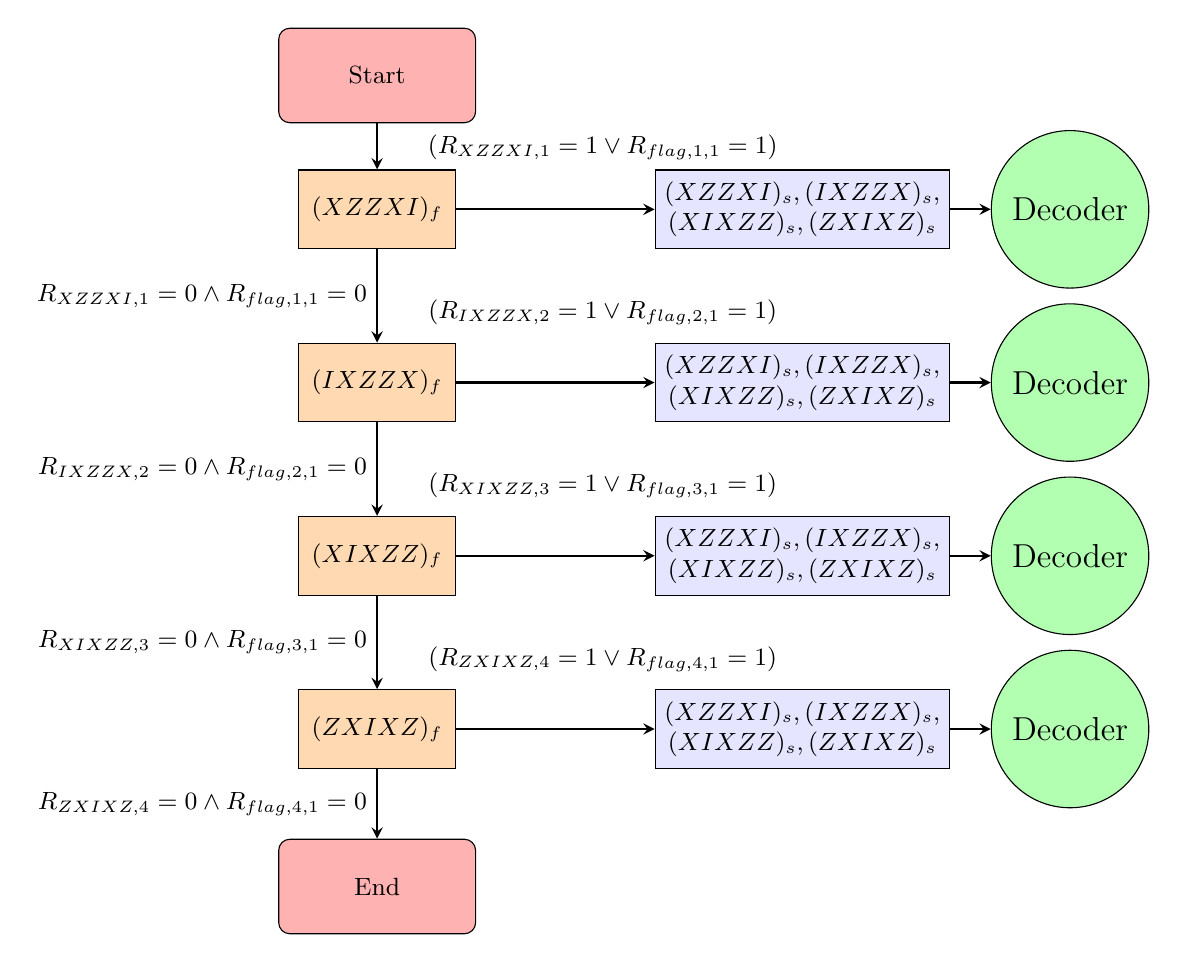
\begin{tikzpicture}[node distance=1.2cm, font=\small] 
        
        % --- 1. Define Styles ---
        \tikzstyle{startstop} = [rectangle, rounded corners, minimum width=2.5cm, minimum height=1.2cm, text centered, draw=black, fill=red!30, font=\small]
        \tikzstyle{raw_syn} = [rectangle, minimum width=2cm, minimum height=1cm, text centered, align=center, draw=black, fill=blue!10, font=\small]
        \tikzstyle{flag_syn} = [rectangle, minimum width=2cm, minimum height=1cm, text centered, align=center, draw=black, fill=orange!30, font=\small]
        \tikzstyle{decode} = [circle, minimum width=2cm, minimum height=1cm, text centered, align=center, draw=black, fill=green!30, font=\large]
        \tikzstyle{arrow} = [thick,->,>=stealth, font=\small]

        % --- 2. Place Nodes ---
        \node (start) [startstop] {Start};
        
        % --- Step 1 ---
        \node (pro1) [flag_syn, below of=start, yshift=-0.5cm] {$(XZZXI)_{f}$};
        \node (pro2b) [raw_syn, right of=pro1, xshift=4.2cm] {$(XZZXI)_s, (IXZZX)_s,$\\$(XIXZZ)_s,(ZXIXZ)_s $};
        \node (decode1) [decode, right of=pro2b, xshift=2.2cm] {Decoder};
        
        % --- Step 2 ---
        \node (pro2a) [flag_syn, below of=pro1, yshift=-1cm] {$(IXZZX)_{f}$};
        \node (pro3b) [raw_syn, right of=pro2a, xshift=4.2cm] {$(XZZXI)_s, (IXZZX)_s,$\\$(XIXZZ)_s,(ZXIXZ)_s $};
        \node (decode2) [decode, right of=pro3b, xshift=2.2cm] {Decoder};

        % --- Step 3 ---
        \node (pro3a) [flag_syn, below of=pro2a, yshift=-1cm] {$(XIXZZ)_{f}$};
        \node (pro4b) [raw_syn, right of=pro3a, xshift=4.2cm] {$(XZZXI)_s, (IXZZX)_s,$\\$(XIXZZ)_s,(ZXIXZ)_s $};
        \node (decode3) [decode, right of=pro4b, xshift=2.2cm] {Decoder};

        % --- Step 4 ---
        \node (pro4a) [flag_syn, below of=pro3a, yshift=-1cm] {$(ZXIXZ)_{f}$};
        \node (pro5b) [raw_syn, right of=pro4a, xshift=4.2cm] {$(XZZXI)_s, (IXZZX)_s,$\\$(XIXZZ)_s,(ZXIXZ)_s $};
        \node (decode4) [decode, right of=pro5b, xshift=2.2cm] {Decoder};

        % End
        \node (stop) [startstop, below of=pro4a, yshift=-0.8cm] {End};

        % --- 3. Draw Arrows ---
        \draw [arrow] (start) -- (pro1);
        
        \draw [arrow] (pro1) -- node[left] {$R_{XZZXI, 1}=0 \wedge R_{flag,1,1}=0$} (pro2a);
        \draw [arrow] (pro1) -- node[above,xshift= 0.6cm, yshift = 0.5cm] {$(R_{XZZXI,1}=1 \vee R_{flag,1,1}=1)$} (pro2b);
        \draw [arrow] (pro2b) -- (decode1);

        % From Step 2
        \draw [arrow] (pro2a) -- node[left] {$R_{IXZZX,2}=0 \wedge R_{flag,2,1}=0$} (pro3a);
        \draw [arrow] (pro2a) -- node[above,xshift= 0.6cm, yshift = 0.6cm] {$(R_{IXZZX,2}=1 \vee R_{flag,2,1}=1)$} (pro3b);
        \draw [arrow] (pro3b) -- (decode2);

        % From Step 3
        \draw [arrow] (pro3a) -- node[left] {$R_{XIXZZ, 3}=0 \wedge R_{flag,3,1}=0$} (pro4a);
        \draw [arrow] (pro3a) -- node[above,xshift= 0.6cm, yshift = 0.6cm] {$(R_{XIXZZ,3}=1 \vee R_{flag,3,1} =1)$} (pro4b);
        \draw [arrow] (pro4b) -- (decode3);
        
        % From Step 4
        \draw [arrow] (pro4a) -- node[above ,xshift= 0.6cm, yshift = 0.6cm] {$(R_{ZXIXZ,4}=1 \vee R_{flag,4,1}=1)$} (pro5b);
        \draw [arrow] (pro4a) -- node[left] {$R_{ZXIXZ, 4}=0 \wedge R_{flag,4,1}=0$} (stop);
        \draw [arrow] (pro5b) -- (decode4);

    \end{tikzpicture}
    \end{adjustbox}
    \caption{Flagged syndrome extraction protocol of $[[5,1,3]]$ adapted from \cite{Chao18}.}
    \label{fig:flowchart}
\end{figure}






\section{Verification}
A flagged syndrome extraction protocol, denoted $Prot$, is defined by a collection of multiple execution paths, $Prot = \{Path_i\}$. Each path $Path_i$ comprises a sequence of syndrome extraction circuits $\{C_{ij}\}$ and a corresponding set of constraints $\Phi_i$ on their measurement outcomes, formulated as $Path_i = (\{C_{ij}\}, \Phi_i)$. 

To verify the overall protocol, we must independently verify each constituent path. For every path, the verification is divided into three distinct steps. The first two steps analyze the properties of the individual syndrome extraction circuits $C_{ij}$ within that specific path's sequence. The third step evaluates the path as a whole, verifying the residual errors on the data qubits after the full sequence of circuits has been executed subject to the classical constraints $\Phi_i$.

\begin{itemize}
    \item \textbf{Step 1 (Verification of syndrome extraction circuits without faults):} We verify that the syndrome extraction qubits in every (flagged) syndrome extraction circuit $C_{ij}$ within the path satisfy Definition~\ref{def:syndrome-extraction-qubit}.
    \item \textbf{Step 2 (Verification of flag qubits under faults):} We verify that for every flagged circuit within the path, the flag qubits satisfy Definition~\ref{def:flag-qubit}. 
    \item \textbf{Step 3 (Verification of protocol distinguishability):} We verify that for the path, the residual error set $\mathcal{E}_{mgs}$ corresponding to each measured generalized syndrome is syndrome-consistent, and that no two residual errors $E_1, E_2 \in \mathcal{E}_{mgs}$ satisfy $E_1 \cdot E_2 \in \mathcal{L} \setminus \mathcal{S}$.
\end{itemize}

\begin{algorithm}[htbp]
\caption{Verification of a Flagged Syndrome Extraction Protocol}
\label{alg:protocol_verification}
\begin{algorithmic}[1]
\Require Protocol $Prot = \{Path_i\}$, where $Path_i = (\{C_{ij}\}, \Phi_i)$
\Ensure \textbf{True} if fault-tolerant, \textbf{False} otherwise

\For{each execution path $Path_i \in Prot$}
    
    \Statex \textbf{Step 1: Syndrome extraction qubits}
    \If{any circuit $C_{ij} \in Path_i$ violates Definition~\ref{def:syndrome-extraction-qubit}}
        \State \Return \textbf{False}
    \EndIf

    \Statex \textbf{Step 2: Flag qubits}
    \If{any flagged circuit $C_{ij} \in Path_i$ violates Definition~\ref{def:flag-qubit}}
        \State \Return \textbf{False}
    \EndIf

    \Statex \textbf{Step 3: Protocol distinguishability}
    \If{the path's resulting $\mathcal{E}_{mgs}$ is not syndrome-consistent \textbf{or} $\exists E_1,E_2 \in \mathcal{E}_{mgs}$ s.t. $E_1 \cdot E_2 \in \mathcal{L} \setminus \mathcal{S}$}
        \State \Return \textbf{False}
    \EndIf

\EndFor

\Statex
\State \Return \textbf{True}
\end{algorithmic}
\end{algorithm}

\paragraph{\textbf{Step 1:(Verification of syndrome extraction circuits without faults)}}
A syndrome extraction circuit is applied to the data qubits and ancilla qubits, and it can be designed with or without flag qubits. To measure one or more Pauli strings, a syndrome extraction circuit utilizes two-qubit gates and measurements on the ancilla and flag qubits. For a syndrome extraction circuit to be considered correct, the measurement outcomes on the ancilla must properly reveal the exact syndrome of the input error on the data qubits in the absence of faults. 

To verify this, we initialize the Pauli representation of the state $Q = Q_1 \dots Q_N$, where $N$ is the total number of qubits involved in the circuit. The data qubit part is $Q_d = Q_{d_1} \dots Q_{d_n}$. Each data qubit $Q_{d_i}$ is assigned two symbolic variables $q_{d_i, x}$ and $q_{d_i, z}$ such that $Q_{d_i} = (q_{d_i, x}, q_{d_i, z})$ to represent arbitrary input errors. Conversely, the ancilla and flag qubits are initialized to $(0, 0)$, as they begin in a known, error-free state. We then symbolically execute the circuit using the semantics described in Section~\ref{sec:quantum computing}. The remaining Pauli error on the data qubits is $E = Q'_{d_1} \dots Q'_{d_n}$, where $Q'_{d_i} = (q'_{d_i, x}, q'_{d_i, z})$. The measurement outcome of the ancilla qubit for each Pauli string $P_k$ measured by the circuit yields a corresponding binary outcome, denoted as $R_{P_k}$.

We must verify that the circuit's measurement results truly match the theoretical calculation derived from the Pauli string $P$. Given a Pauli string $P = (P_{1,x}, P_{1,z}) \dots (P_{n,x}, P_{n,z})$ acting on the $n$ data qubits, we compute the Boolean commutation relation between the data qubit errors $E$ and the Pauli string $P$ as follows:

\begin{equation}
S_{P,E} = \bigoplus_{i=1}^n \big( ( q_{d_i, x} \land P_{i,z}) \oplus (q_{d_i, z} \land P_{i,x}) \big)
\end{equation}

A result of $S_{P,E} = 1$ indicates that the Pauli error $E$ on the data qubits and the Pauli string $P$ anti-commute, while $0$ indicates that they commute. For a syndrome extraction circuit, we want to verify that all measurement results corresponding to each Pauli string are correct. To achieve this, we feed the following constraint to the SAT solver to search for counterexamples:

\begin{equation}
\mathrm{Constraint}_{\mathrm{total}} = \bigvee_k (R_{P_k} \neq S_{P_k,E})
\end{equation}


\begin{lemma}
    For a (flagged) syndrome extraction circuit $C$ correspond to a set of stabilizers ${P_k}$ is the result of $\mathrm{Constraint}_{\mathrm{total}}$ is \texttt{UNSAT} $\Leftrightarrow C$ satisfies Def. \ref{def:syndrome-extraction-circuit}.
\end{lemma}
If the solver returns \texttt{sat}, it means there exists a valid configuration where the measurement outcome of the syndrome extraction circuit does \emph{not} match the direct calculation from the Pauli string, indicating a flaw in the circuit. Conversely, a result of \texttt{unsat} proves the circuit's functional correctness under fault-free conditions. We systematically check all syndrome extraction circuits utilized in the flagged syndrome extraction protocol.

\paragraph{\textbf{Example}}
Verifying Step 1 of the syndrome extraction circuit for the Pauli string $P=XZZXI$ requires five data qubits and one ancilla qubit prepared in the $X$-basis, denoted collectively as $Q = Q_{d_1} Q_{d_2} Q_{d_3} Q_{d_4} Q_{d_5} Q_{ancX}$. Each data qubit is initialized as $Q_{d_i} = (q_{d_i,x}, q_{d_i,z})$, and the ancilla qubit is initialized as $Q_{ancX} = (0,0)$. The circuit and the corresponding symbolic execution results are shown in Fig.~\ref{fig:step1_example}, where $R_{XZZXI}$ represents the measurement outcome of the ancilla qubit. Because the ancilla $Q_{ancX}$ is prepared and measured in the $X$-basis, the measurement outcome $R_{XZZXI}$ directly corresponds to the $Z$ component of the final ancilla state, $Q'_{ancX}$. 

\begin{figure}[htbp]
    \centering
    % adjustbox ensures it fits perfectly without shrinking unless absolutely necessary
    \begin{adjustbox}{max width=\textwidth}
    % Adding \large here forces all text inside the quantum circuit to jump up in size
    \large
    \begin{quantikz}[row sep=0.5cm, column sep=0.4cm]
        % Row 1
        \lstick{$Q_{d_1} = (q_{d_1, x}, q_{d_1,z})$} & \qw & \targ{}   & \qw        & \qw        & \qw       & \qw & \qw & \qw \rstick{$Q'_{d_1} = (q_{d_1, x}, q_{d_1,z})$}  \\
        % Row 2 
        \lstick{$Q_{d_2} = (q_{d_2, x}, q_{d_2,z})$} & \qw & \qw       & \ctrl{4}   & \qw        & \qw       & \qw & \qw & \qw \rstick{$Q'_{d_2} = (q_{d_2, x}, q_{d_2,z})$}  \\
        % Row 3
        \lstick{$Q_{d_3}= (q_{d_3, x}, q_{d_3,z})$}  & \qw & \qw       & \qw        & \ctrl{3}   & \qw       & \qw & \qw & \qw \rstick{$Q'_{d_3}= (q_{d_3, x}, q_{d_3,z})$} \\
        % Row 4
        \lstick{$Q_{d_4}= (q_{d_4, x}, q_{d_4,z})$}  & \qw & \qw       & \qw        & \qw        & \targ{}   & \qw & \qw & \qw \rstick{$Q'_{d_4}= (q_{d_4, x}, q_{d_4,z})$} \\
        % Row 5
        \lstick{$Q_{d_5}= (q_{d_5, x}, q_{d_5,z})$}  & \qw & \qw       & \qw        & \qw        & \qw       & \qw & \qw & \qw \rstick{$Q'_{d_5}= (q_{d_5, x}, q_{d_5,z})$}  \\
        % Row 6 (Ancilla)
        % The long equation is now split into two lines using an array, keeping the circuit narrow!
        \lstick{$Q_{ancX} = (0, 0)$}                & \qw & \ctrl{-5} & \control{} & \control{} & \ctrl{-2} & \ \push{\begin{array}{l} Q'_{ancX} = (Q'_{ancX,x} = 0, \\ Q'_{ancX,z} = q_{d_1,z} \oplus q_{d_2, x} \oplus q_{d_3, x} \oplus q_{d_4,z}) \end{array}} & \meter{X} & \rstick{$R_{XZZXI} = Q'_{ancX,z}$}
    \end{quantikz}
    \end{adjustbox}
    \caption{Example of a syndrome extraction circuit.}
    \label{fig:step1_example}
\end{figure}

To map the relationship between the input Pauli error $E = (q_{d_1, x}, q_{d_1,z}) \dots (q_{d_5, x}, q_{d_5,z})$ and the Pauli string $P = XZZXI$, which is represented as $(1,0)(0,1)(0,1)(1,0)(0,0)$, we calculate:
\begin{align*}
S_{XZZXI,E} &= \big( (q_{d_1, x} \land 0) \oplus (q_{d_1, z} \land 1) \big) \oplus \\
          &\quad \big( (q_{d_2, x} \land 1) \oplus (q_{d_2, z} \land 0) \big) \oplus \\
          &\quad \big( (q_{d_3, x} \land 1) \oplus (q_{d_3, z} \land 0) \big) \oplus \\
          &\quad \big( (q_{d_4, x} \land 0) \oplus (q_{d_4, z} \land 1) \big) \oplus \\
          &\quad \big( (q_{d_5, x} \land 0) \oplus (q_{d_5, z} \land 0) \big)  \\
          &= (q_{d_1, z} \land 1) \oplus (q_{d_2, x} \land 1) \oplus (q_{d_3, x} \land 1) \oplus (q_{d_4, z} \land 1) \\
          &= q_{d_1, z} \oplus q_{d_2, x} \oplus q_{d_3, x} \oplus q_{d_4, z}
\end{align*}

We then add the following constraint to the SAT solver to verify the result:
\begin{equation}
\mathrm{Constraint}_{\mathrm{total}} = \big( R_{XZZXI} \neq S_{XZZXI,E} \big)
\end{equation}

If the solver returns \texttt{unsat}, it guarantees that the extraction circuit for $XZZXI$ yields the correct syndrome under fault-free conditions.


\paragraph{\textbf{Step 2: Verification of flag qubits under faults}}
In this step, we verify that the flag qubit functions correctly by using  SAT solver. The flag qubit is designed to detect whether a high-weight error has occurred. A valid flag qubit must yield a \texttt{True} measurement outcome whenever a $t$-fault event causes an error $E$ on the data qubits such that $\mathrm{wt}_{\min}(E) > t$. 

To verify this property, we initialize the Pauli representation of the state $Q = Q_1 \dots Q_N$, where $N$ is the total number of qubits involved in the circuit. All qubits are initialized to $(0,0)$, representing an error-free initial state. We then symbolically execute the flagged syndrome extraction circuit under the presence of faults. Faults are introduced by adding Boolean variables that represent Pauli errors injected on the qubits after each gate operation. Because we only consider two-qubit gates, when a two qubit gate acts on a control qubit $Q_c = (Q_{c,x}, Q_{c,z})$ and a target qubit $Q_t = (Q_{t,x}, Q_{t,z})$, we inject a Pauli error $(e_{c,x}, e_{c,z})$ on $Q_c$ and $(e_{t,x}, e_{t,z})$ on $Q_t$. The resulting state becomes:

\begin{equation}
    Q'_c = (Q_{c,x} \oplus e_{c,x}, Q_{c,z} \oplus e_{c,z}) , \quad
    Q'_t = (Q_{t,x} \oplus e_{t,x}, Q_{t,z} \oplus e_{t,z})
\end{equation}

Modeling these two-qubit gate faults is sufficient for the noise model defined in Section~\ref{sec:quantum computing}. Other fault mechanisms (such as state preparation or measurement errors) manifest as single-qubit errors, which are equivalent to errors arising from a two-qubit gate fault, as illustrated in Fig.~\ref{equivalence_of_fault}. 

\begin{figure}[htbp]
  \centering
  
  % --- First Subfigure: Stacked to full width ---
  \begin{subfigure}{\textwidth}
    \centering
    \begin{adjustbox}{max width=\textwidth}
    \begin{quantikz}[column sep=0.3cm]
        \lstick{$Q_1$} & \gate[2]{\text{2Q gate}} & \gate[, style={draw=red}]{E} \gategroup[1, steps=1, style={dashed, rounded corners, fill=red!20, inner xsep=2pt}, background]{fault} & \gate[2]{\text{2Q gate}} & \qw \\
        \lstick{$Q_2$} &                           & \qw                                                         &                           & \qw 
    \end{quantikz}
    =
    \begin{quantikz}[column sep=0.3cm]
        \lstick{$Q_1$} & \gate[2]{\text{2Q gate}} & \gate[2]{\text{2Q gate}} \gategroup[2, steps=2, style={dashed, rounded corners, fill=blue!20, inner xsep=2pt}, background]{2Q gate fault} & \gate[, style={draw=blue}]{E} & \qw \\
        \lstick{$Q_2$} &                           &                                                         & \gate[, style={draw=blue}]{E} & \qw 
    \end{quantikz}
    =
    \begin{quantikz}[column sep=0.3cm]
        \lstick{$Q_1$} & \gate[2]{\text{2Q gate}} \gategroup[2, steps=2, style={dashed, rounded corners, fill=blue!20, inner xsep=2pt}, background]{2Q gate fault} & \gate[, style={draw=blue}]{E} & \gate[2]{\text{2Q gate}} & \qw \\
        \lstick{$Q_2$} &                           & \gate[, style={draw=blue}]{E} &                           & \qw     
    \end{quantikz}
    \end{adjustbox}
    \subcaption{Equivalence of error caused by a fault on one qubit and a two-qubit gate fault.}
    \label{fig:idle-2q-error-equivalence}
  \end{subfigure}
  
  \vspace{0.6cm} % Adds breathing room between the stacked subfigures
  
  % --- Second Subfigure: Stacked to full width ---
  \begin{subfigure}{\textwidth}
    \centering
    \begin{adjustbox}{max width=0.8\textwidth}
    \begin{quantikz}[column sep=0.5cm]
    \lstick{$Q_1$} & \gate[2]{\text{2Q gate}} & \qw & \qw \\
    \lstick{$Q_2$} &                           & \gate[, style={draw=red}]{E} \gategroup[1, steps=2, style={dashed, rounded corners, fill=red!20, inner xsep=8pt}, background, label style={xshift=0.2cm}]{measurement fault} & \meter{}
\end{quantikz}
    =
    \begin{quantikz}[column sep=0.5cm]
        \lstick{$Q_1$} & \gate[2]{\text{2Q gate}} \gategroup[2, steps=2, style={dashed, rounded corners, fill=blue!20, inner xsep=2pt}, background]{2Q gate fault} & \qw & \qw \\
        \lstick{$Q_2$} &                           & \gate[, style={draw=blue}]{E} & \meter{}
    \end{quantikz}
    \end{adjustbox}
    \subcaption{Equivalence of the errors caused by measurement and a 2Q gate fault.}
    \label{fig:meas-2q-error-equivalence}
  \end{subfigure}

  % --- Main Figure Caption ---
  \caption{Demonstration of fault equivalence in two-qubit gates.}
  \label{equivalence_of_fault}
\end{figure}
For a $t$-fault event, we add a constraint to bound the total number of injected gate faults. Let $e_p$ be a Boolean indicator  for the $p$-th two-qubit gate. A fault occurs if any of the variables representing  Pauli error induced by that  gate evaluate to \texttt{True}. Therefore, $e_p$ is defined as the logical OR of these variables:
\begin{equation}
e^{p} = e_{c,x}^{p} \lor e_{c,z}^{p} \lor e_{t,x}^{p} \lor e_{t,z}^{p}
\end{equation}

The $t$-fault condition is then enforced by constraining the sum of all $e_p$ variables across the $m$ gates in the circuit to be exactly $t$:

\begin{equation}
\mathrm{Constraint}_{\mathrm{fault}} : \sum_{p=1}^{m} e^{p}= t
\end{equation}
The constraint is encoded using Z3's pseudo-Boolean support~\cite{Z3}, transformed into a SAT problem ~\cite{pseudo_bool_article}, and then solved with CryptoMiniSat~\cite{cryptominisat}.
After the symbolic execution of the entire circuit, the measurement outcomes of the flag qubits $\{R_{flag,j}\}$ are formulas of the Boolean variables $e^{p}_{c/t, x/z}$, accounting for architectures that may contain multiple flag qubits. The constraint of ``no flag is raised'' is:
\begin{equation}
\mathrm{Constraint_{flag}} = \bigwedge_{j} \mathrm{Not}(R_{flag,j})
\end{equation}

Finally, the Pauli operator of the data qubits after symbolic execution of the flagged syndrome extraction circuit, $Q'_d$, represents the total accumulated Pauli error $E$ remaining on the data block:
\begin{equation}
E = Q'_{d_1}  \dots Q'_{d_n}, \quad Q'_{d_i} = (Q'_{d_i,x}, Q'_{d_i,z})
\end{equation}
Each $Q'_{d_i, x/z}$ are Boolean formula of  $e^{p}_{c/t, x/z}$.
To determine the minimum weight $\mathrm{wt}_{\min}(E)$, we must consider all degenerate errors equivalent to $E$, which is $E \cdot S$ for any stabilizer $S$ in the stabilizer group $\mathcal{S} = \langle G_1, \dots, G_{n-k} \rangle$ of the QECC. 


We can efficiently encode any stabilizer $S \in \mathcal{S}$ using $n-k$ Boolean variables. For example, consider a quantum error-correcting code (QECC) on three qubits with two stabilizer generators, $\mathcal{S} = \langle G_1, G_2 \rangle = \langle Z_1Z_2, Z_2Z_3 \rangle$. These generators are represented as:

{\small
\begin{equation*}
\begin{aligned}
G_1 &= (G_{1,1,x}, G_{1,1,z})(G_{1,2,x}, G_{1,2,z})(G_{1,3,x}, G_{1,3,z}) = (0,1)(0,1)(0,0) \to Z_1Z_2 \\
G_2 &= (G_{2,1,x}, G_{2,1,z})(G_{2,2,x}, G_{2,2,z})(G_{2,3,x}, G_{2,3,z}) = (0,0)(0,1)(0,1) \to Z_2Z_3
\end{aligned}
\end{equation*}
}

By introducing two  Boolean variables $\{c_{G_1}, c_{G_2}\}$, we can represent any stabilizer as the product $S = {G_1}^{c_{G_1}} \cdot {G_2}^{c_{G_2}}$.  $S$ is computed as :

{\small
\begin{equation*}
\begin{aligned}
G_1^{c_{G_1}} &= (0 \land c_{G_1}, 1 \land c_{G_1})(0 \land c_{G_1}, 1 \land c_{G_1})(0 \land c_{G_1}, 0 \land c_{G_1}) = (0, c_{G_1})(0, c_{G_1})(0, 0) \\
G_2^{c_{G_2}} &= (0 \land c_{G_2}, 0 \land c_{G_2})(0 \land c_{G_2}, 1 \land c_{G_2})(0 \land c_{G_2}, 1 \land c_{G_2}) = (0, 0)(0, c_{G_2})(0, c_{G_2}) \\
\Rightarrow S &= G_1^{c_{G_1}} \cdot G_2^{c_{G_2}} = (0, c_{G_1}) (0, c_{G_1} \oplus c_{G_2}) (0, c_{G_2}) =S_1S_2S_3
\end{aligned}
\end{equation*}
}

The valuation of these variables enumerates the entire stabilizer group $\mathcal{S}$. For instance, if $(c_{G_1}, c_{G_2}) = (1,1)$, then $S = Z_1Z_2 \cdot Z_2Z_3 = Z_1Z_3$. In general, the Pauli operator on the $i$-th qubit of any stabilizer $S = S_1 \dots S_n \in \mathcal{S}$ is encoded using the following summation:

\begin{equation}
S_i = (S_{i,x}, S_{i,z}) = \left( \bigoplus_{l=1}^{n-k} ( G_{l,i,x} \land c_{G_l}), \bigoplus_{l=1}^{n-k} ( G_{l,i,z} \land c_{G_l}) \right)
\end{equation}

where $(G_{l,i,x}, G_{l,i,z})$ denotes the binary components of the $i$-th qubit of the $l$-th stabilizer generator $G_l$.
All degenerate errors $E \cdot S$ can then be represented by the bitwise XOR of the binary representations of the error $E$ and the stabilizer $S$:

\begin{equation}
(ES)_i = (Q'_{d_i, x} \oplus S_{i,x}, Q'_{d_i, z} \oplus S_{i,z})
\end{equation}

To determine if the minimum weight of the error $\mathrm{wt}_{\min}(E)$ is strictly greater than $t$, we must verify that the weight of the Pauli operator $ES$ exceeds $t$ for every possible stabilizer $S$ in the group $\mathcal{S}$. This requirement is expressed by a conjunction over all $n-k$ Boolean generator coefficients $c_{G_l}$:

\begin{equation}
\mathrm{Constraint}_{\mathrm{error}} = \bigwedge_{\{c_{G_1}, \dots , c_{G_{n-k}}\} \in \{0,1\}^{n-k}} \left( \sum_{i=1}^{n} \Big( (Q'_{d_i, x} \oplus S_{i,x}) \lor (Q'_{d_i, z} \oplus S_{i,z}) \Big) > t \right)
\end{equation}
For this constraint we can also transform this constraint to SAT problem from pseudo Boolean constraint as we did for $\mathrm{Constraint}_{\mathrm{fault}}$ .
We combine all of the constraints together to form the final satisfiability query:

\begin{equation}
\mathrm{Constraint}_{\mathrm{total}} : \mathrm{Constraint}_{\mathrm{fault}} \land \mathrm{Constraint}_{\mathrm{flag}} \land \mathrm{Constraint}_{\mathrm{error}}
\end{equation}


\begin{lemma}
    For a  flagged syndrome extraction circuit $C$ correspond to a set of stabilizers ${P_k}$ is the result of $\mathrm{Constraint}_{\mathrm{total}}$ is \texttt{UNSAT} and also passed step 1 $\Leftrightarrow C$ satisfies Def. \ref{def:flagged-syndrome-circuit}.
\end{lemma}
We use an SAT solver to verify this combined formula. If the solver returns \texttt{sat} , it means that there exists a $t$-fault event that does not raise any flag qubits but results in a data error with a minimum weight strictly greater than $t$. This indicates that the flagged syndrome extraction circuit fails to function as required. Conversely, if the result is \texttt{unsat} , the circuit is formally verified to be safe against all such $t$-fault events.



\paragraph{\textbf{Example}}
We consider a flagged syndrome extraction circuit for the Pauli string $P = XZZXI$ of a $[[5,1,3]]$ QECC as shown in Fig.~\ref{fig:step2_example_a}. There are five data qubits, one ancilla qubit prepared in the $X$-basis and one flag qubit prepared in the $Z$-basis, denoted collectively as $$Q = Q_{d_1} Q_{d_2} Q_{d_3}Q_{d_4} Q_{d_5} Q_{ancX} Q_{flagZ}$$. In Fig.~\ref{fig:step2_example_b}, we show the partial symbolic execution of the flagged syndrome extraction circuit of $P=XZZXI$. After this symbolic execution, we obtain the Pauli error on data qubits  $E = Q'_{d_1} Q'_{d_2}Q'_{d_3}Q'_{d_4}Q'_{d_5}$ and the flag qubit measurement output $R_{flag,1} = Q'_{flagZ, x}$ (we do not need syndrome measurement outcome $R_{XZZXI}$ in this step), where each $Q'_{i,x/z}$ and $R_{flag,1} $ is a formula composed of the injected fault variables $e^{p}_{c/t, x/z}$. Since there are six gates and $t = \lfloor \frac{3-1}{2} \rfloor = 1$, we can establish:

\begin{equation}
\mathrm{Constraint}_{\mathrm{fault}} : \sum_{p=1}^{6} e^{p}= 1 , \quad \mathrm{Constraint}_{\mathrm{flag}}: \mathrm{Not}(R_{flag,1})
\end{equation}

For the $[[5,1,3]] $ QECC, the stabilizer group is $\mathcal{S} = \langle G_1= XZZXI, G_2 = IXZZX , G_3= XIXZZ, G_4 = ZXIXZ \rangle$, so we can use four variables $c_{G_1}, c_{G_2}, c_{G_3}, c_{G_4}$ to represent all the stabilizers:
\begin{equation}
\begin{aligned}
S = \big( & (c_{G_1} \oplus c_{G_3}, c_{G_4}), \\
       & (c_{G_2} \oplus c_{G_4}, c_{G_1}), \\
       & (c_{G_3}, c_{G_1} \oplus c_{G_2}), \\
       & (c_{G_1} \oplus c_{G_4}, c_{G_2} \oplus c_{G_3}), \\
       & (c_{G_2}, c_{G_3} \oplus c_{G_4}) \big)
\end{aligned}
\end{equation}
Since we have $E$ and $S$, we can encode all the degenerate errors $E \cdot S$ and trivially obtain $\mathrm{Constraint}_{\mathrm{error}}$. We then pass the conjunction of  constraints $\mathrm{Constraint}_{\mathrm{fault}},  \mathrm{Constraint}_{\mathrm{flag}}$,and $\mathrm{Constraint}_{\mathrm{error}}$to  SAT solver.
The result  is \texttt{unsat} which means that there is no fault will cause error with minimum weight greater than $t $ and doesn't triggers flag qubit.
\begin{figure}[h]
    \centering
    
    % --- Subfigure (a) ---
    \begin{subfigure}{\linewidth}
    \centering
    \scalebox{1}{ % <-- Adjust this number to scale the first circuit
    \begin{quantikz}[row sep=0.4cm, column sep=0.25cm, wire types={q,q,q,q,q,q,q,n}]
        % Row 1
        & \qw & \targ{}   & \qw        & \qw        & \qw        & \qw       & \qw         & \qw \\
        % Row 2 
        & \qw & \qw       & \qw        & \ctrl{4}   & \qw        & \qw       & \qw         & \qw \\
        % Row 3
        & \qw & \qw       & \qw        & \qw        & \ctrl{3}   & \qw       & \qw         & \qw \\
        % Row 4
        & \qw & \qw       & \qw        & \qw        & \qw        &\qw        & \targ{}     & \qw \\
        % Row 5
        & \qw & \qw       & \qw        & \qw        & \qw        & \qw       & \qw         & \qw \\
        % Row 6 (Ancilla)
        & \qw & \ctrl{-5} & \ctrl{1}   & \control{} & \control{} & \ctrl{1}  & \ctrl{-2}   & \meter{$X$} \\
        % Row 7 (Flag)
        & \qw & \qw       & \targ{}    & \qw        & \qw        & \targ{}   & \qw         & \meter{$Z$} \\
        % Row 8 (Gate Labels)
        &     & \push{\text{gate}^{1}} & \push{\text{gate}^{2}} & \push{\text{gate}^{3}} & \push{\text{gate}^{4}} & \push{\text{gate}^{5}} & \push{\text{gate}^{6}} & 
    \end{quantikz}
    }
    \caption{Flagged syndrome extraction circuit of $XZZXI$}
    \label{fig:step2_example_a}
    \end{subfigure}

    \vspace{0.5em}

    % --- Subfigure (b) ---
    \begin{subfigure}{\linewidth}
    \centering
    \scalebox{0.77}{ % <-- Adjust this number to scale the second circuit
    \begin{quantikz}[row sep=0.4cm, column sep=0.1cm]
        % Row 1
        \lstick{$Q_{d_1} = (0,0)$} & \qw & \targ{}   & \push{(e^{1}_{t,x}, e^{1}_{t,z})} & \qw  & \qw  & \push{(e^{1}_{t,x}, e^{1}_{t,z})}  & \qw &  \push{(e^{1}_{t,x}, e^{1}_{t,z})} & \ \ldots \ &  \ \push{\begin{array}{c} Q'_{d_1} =  (Q'_{d_1,x}, Q'_{d_1, z}) \end{array}} \\
        % Row 2 
        \lstick{$Q_{d_2} =  (0,0)$} & \qw & \qw       & \push{(0,0)} & \qw  & \qw  & \push{(0,0)} & \ctrl{4} & \push{\begin{array}{c} (e^{3}_{c,x}, \\ e^{1}_{c,x} \oplus e^{2}_{c,x} \oplus e^{3}_{c,z}) \end{array}} & \ \ldots \ & \ \push{\begin{array}{c} Q'_{d_2} =  (Q'_{d_2,x}, Q'_{d_2, z}) \end{array}} \\
        % Row 3
        \lstick{$Q_{d_3}=  (0,0)$}  & \qw & \qw       & \push{(0,0)} & \qw  & \qw  & \push{(0,0)} & \qw  & \push{(0,0)}  & \ \ldots \  &  \ \push{\begin{array}{c} Q'_{d_3} =  (Q'_{d_3,x}, Q'_{d_3, z}) \end{array}}\\
        % Row 4
        \lstick{$Q_{d_4}=  (0,0)$}  & \qw & \qw       & \push{(0,0)} & \qw  & \qw   & \push{(0,0)} & \qw & \push{(0,0)} & \ \ldots \ &  \ \push{\begin{array}{c} Q'_{d_4} =  (Q'_{d_4,x}, Q'_{d_4, z}) \end{array}} \\
        % Row 5
        \lstick{$Q_{d_5}=  (0,0)$}  & \qw & \qw       & \push{(0,0)} & \qw  & \qw   & \push{(0,0)}& \qw & \push{(0,0)}  & \ \ldots \ & \  \push{\begin{array}{c} Q'_{d_5} =  (Q'_{d_5,x}, Q'_{d_5, z}) \end{array}} \\
        % Row 6 (Ancilla)
        \lstick{$Q_{ancX} = (0, 0)$} & \qw & \ctrl{-5} & \push{(e^{1}_{c,x}, e^{1}_{c,z})} & \qw  &\ctrl{1}  &\push{\begin{array}{c} (e^{1}_{c,x} \oplus e^{2}_{c,x} , \\ e^{1}_{c,z} \oplus e^{2}_{c,z}) \end{array}} & \control{} & \push{\begin{array}{c} (e^{1}_{c,x} \oplus e^{2}_{c,x} \oplus e^{3}_{t,x}, \\ e^{1}_{c,z} \oplus e^{2}_{c,x} \oplus e^{3}_{t,z}) \end{array}}  & \ \ldots \ &  \ \push{\begin{array}{c} (Q'_{ancX,x}, \\ Q'_{ancX, z}) \end{array}} & \meter{X} & \rstick{$R_{XZZXI} =  Q'_{ancX, z}$} \\
        % Row 7 (Flag)
        \lstick{$Q_{flagZ} = (0, 0)$} & \qw & \qw       & \push{(0,0)} & \qw  &\targ{}   &\push{\begin{array}{c} (e^{1}_{c,x} \oplus e^{2}_{t,x}, \\ e^{2}_{t,z}) \end{array}} & \qw  &\push{\begin{array}{c} (e^{1}_{c,x} \oplus e^{2}_{t,x}, \\ e^{2}_{t,z}) \end{array}}  & \ \ldots \ &  \ \push{\begin{array}{c} (Q'_{flagZ,x}, \\ Q'_{flagZ, z}) \end{array}}  & \meter{Z} & \rstick{$R_{flag,1} = Q'_{flagZ, x}$}
    \end{quantikz}
    }
    \caption{Symbolic execution of the flagged syndrome extraction circuit of $XZZXI$}
    \label{fig:step2_example_b}
\end{subfigure}

    \caption{Example of Step 2.}
    \label{fig:step2_example}
\end{figure}


\paragraph{\textbf{Step 3: Verification of the distinguishability of the flagged syndrome extraction protocol}}

For each path $Path_i$  there could be different fault events  that correspond to the same measure generalized syndrome  $mgs$ and the correspond error set $\mathcal{E}_{mgs}$. Since there are two conditions for a path in the flagged syndrome extraction protocol to terminate as Prop. \ref{prop:termination}.  We want to check that 
\begin{enumerate}
    \item $\mathcal{E}_{mgs}$ is syndrome-consistent 
    \item $\forall E_1, E_2 \in \mathcal{E}_{mgs}, E_1 \cdot E_2 \in \mathcal{S}$ 
\end{enumerate}
Since for each path every  $\mathcal{E}_{mgs}$ satisfies (1) is valid, by lemma \ref{lemma:decoder} there exist  a decoder. With (2) then by Thm.\ref{thm:mains} the syndrome extraction protocol along with the decoder is a FTEC.  


To a path, we initialize the Pauli state $Q = Q_1 \dots Q_N$ to $(0,0)$, representing an initial state  symbolically then  run the circuits with injected faults as described in Step 2. We define the fault indicator variable $e^p$ for the $p$-th gate as:

\begin{equation}
e^{p} = e_{c,x}^{p} \lor e_{c,z}^{p} \lor e_{t,x}^{p} \lor e_{t,z}^{p}
\end{equation}

The $t$-fault condition is then enforced by constraining the sum of all $e_p$ variables across the $m$ gates in the circuit to be exactly $t$:

\begin{equation}
\mathrm{Constraint}_{\mathrm{fault}}  = \sum_{p=1}^{m} e^{p}= t
\end{equation}
We will also transform this constraint to SAT problem from pseudo Boolean constraint as we did in step 2.

For each path, we introduce a Boolean formula $\Phi$ to record the branching conditions between circuits. 
\begin{equation}
\mathrm{Constraint}_{\mathrm{path}} : \Phi
\end{equation}


In path 2  Fig.~\ref{fig:flowchart_path_2} which is a part of the Fig. ~\ref{fig:flowchart} the path condition $\Phi$ is  constructed as follows: the protocol first executes the circuit $(XZZXI)_f$ in the first round, yielding the result $(R_{XZZXI,r1} = 0 \land R_{flag,r1,1} = 0)$. It then executes $(IXZZX)_f$ in the second round, yielding $(R_{IXZZX,r2} = 1 \lor R_{flag,r2,1} = 1)$, before finally executing the syndrome extraction circuits for all stabilizers in the last round. Consequently, the path constraint is defined as:
\begin{equation}
\Phi = (R_{XZZXI,r1} = 0 \land R_{flag,r1,1} = 0) \land (R_{IXZZX,r2} = 1 \lor R_{flag,r2,1} = 1)
\end{equation}




\begin{figure}[h]
    \centering
    % Changed back to \textwidth so LaTeX stops shrinking your fonts!
    \begin{adjustbox}{max width=\textwidth}
    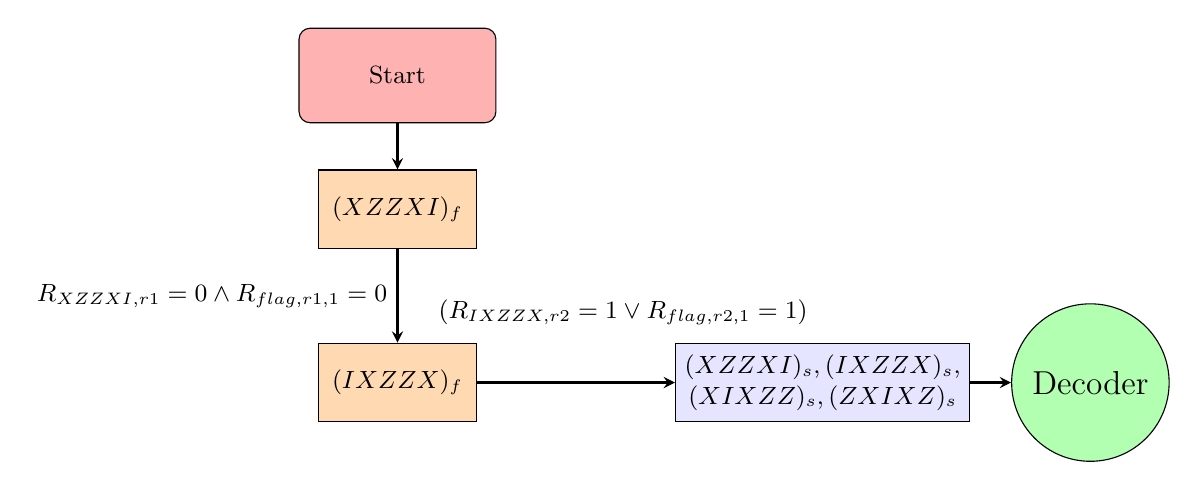
\begin{tikzpicture}[node distance=1.2cm, font=\mid] 
        
        % --- 1. Define Styles (Upgraded to \Large, slightly reduced minimum widths) ---
        \tikzstyle{startstop} = [rectangle, rounded corners, minimum width=2.5cm, minimum height=1.2cm, text centered, draw=black, fill=red!30, font=\small]
        \tikzstyle{raw_syn} = [rectangle, minimum width=2cm, minimum height=1cm, text centered, align=center, draw=black, fill=blue!10, font=\small]
        \tikzstyle{flag_syn} = [rectangle, minimum width=2cm, minimum height=1cm, text centered, align=center, draw=black, fill=orange!30, font=\small]
        \tikzstyle{decode} = [circle, minimum width=2cm, minimum height=1cm, text centered, align=center, draw=black, fill=green!30, font=\large]
        \tikzstyle{arrow} = [thick,->,>=stealth, font=\small] % Arrow math slightly smaller so it fits the lines

        % --- 2. Place Nodes ---
        \node (start) [startstop] {Start};
        
        % --- Step 1 ---
        \node (pro1) [flag_syn, below of=start, yshift=-0.5cm] {$(XZZXI)_{f}$};
        % Tightened xshift to 4.2cm so the diagram fits on the page naturally
        
        \node (pro2a) [flag_syn, below of=pro1, yshift=-1cm] {$(IXZZX)_{f}$};
        \node (pro3b) [raw_syn, right of=pro2a, xshift=4.2cm] {$(XZZXI)_s, (IXZZX)_s,$\\$(XIXZZ)_s,(ZXIXZ)_s $};
        \node (decode2) [decode, right of=pro3b, xshift=2.2cm] {Decoder};

        % --- 3. Draw Arrows ---
        \draw [arrow] (start) -- (pro1);
        \draw [arrow] (pro1) -- node[left] {$R_{XZZXI, r1}=0 \wedge R_{flag,r1,1}=0$} (pro2a);
        \draw [arrow] (pro2a) -- node[above,xshift= 0.6cm, yshift = 0.6cm] {$(R_{IXZZX,r2}=1 \vee R_{flag,r2,1}=1)$} (pro3b);
        \draw [arrow] (pro3b) -- (decode2);
    \end{tikzpicture}
    \end{adjustbox}
    \caption{path 2 of Fig.~\ref{fig:flowchart}}
    \label{fig:flowchart_path_2}
\end{figure}



 

In each path, the measurement outcomes collected from the ancilla and flag qubits constitute a measured generalized syndrome, denoted as $mgs$. To verify the protocol's correctness, we must ensure that no two distinct $t$-fault events can produce the same generalized syndrome while resulting in non-degenerate data errors $E$. 

To model two distinct fault events simultaneously within a single SAT query, we instantiate two independent copies of the entire symbolic execution logic. Specifically, we duplicate every Boolean formula and state variable derived in the previous steps—including all intermediate qubit representations, $\mathrm{Constraint}_{\mathrm{path}}$, $\mathrm{Constraint}_{\mathrm{fault}}$, and $\mathrm{Constraint}_{\mathrm{last\_syndrome}}$. We distinguish these two instances by replacing the fault variables $e^{p}_{c/t, x/z}$ with two independent sets: $\{e^{p(1)}_{c/t, x/z}\}$ and $\{e^{p(2)}_{c/t, x/z}\}$. 

Consequently, every symbolic state and measurement result is tracked in two versions:
\begin{itemize}
    \item \textbf{Instance 1:} Uses fault variables $e^{p(1)}$, resulting in qubit states $Q^{(1)}$, a generalized syndrome $mgs^{(1)}$, and a final data error $E^{(1)}$.
    \item \textbf{Instance 2:} Uses fault variables $e^{p(2)}$, resulting in qubit states $Q^{(2)}$, a generalized syndrome $mgs^{(2)}$, and a final data error $E^{(2)}$.
\end{itemize}


The  $mgs^{(1)}$ and $mgs^{(2)}$ are  the measured generalized syndromes produced by the two different $t$-fault events, respectively. The constraint enforcing that the generalized syndromes are identical is:

\begin{equation}
\mathrm{Constraint}_{\mathrm{syn\_gen}} : \left( mgs^{(1)} = mgs^{(2)} \right)
\end{equation}

Since each path in the protocol will meet one of the two conditions we stated in Prop. \ref{prop:termination}, we will consider the two condition separately.

\subparagraph{\textbf{Condition 1} }
For this case the protocol stops when the path has at least $t$ faults for the correspond error set $\mathcal{E}_{mgs}$ we have to verify the set is syndrome consistent which means there are no two errors $E_1 , E_2 \in \mathcal{E}_{mgs}$ has different ideal syndrome or $E_1 \cdot E_2 \notin \mathcal{S}$(non-degenerate).


To determine whether the remaining Pauli error on data qubits $E^{(1)}$ and $E^{(2)}$ are non-degenerate, we check if their product $E^{(1)+(2)} = E^{(1)} \cdot E^{(2)}$ lies outside the stabilizer group $\mathcal{S}$. We rely on the following lemma:

\begin{lemma}
For a QECC with a stabilizer group $\mathcal{S} = \langle G_1, \dots, G_{n-k} \rangle$ and logical operators $\mathcal{L} = \{\bar{X}_1, \dots, \bar{X}_k, \bar{Z}_1, \dots, \bar{Z}_k\}$, if a Pauli string $P$ commutes with all generators $G_i$ and all logical operators $\bar{X}_j, \bar{Z}_j$, then $P$ lies in the group $\mathcal{S}$ (up to an overall phase).
\end{lemma}

We calculate the Boolean commutation relation $S_{P, E^{(1)+(2)}}$ between the combined error $E^{(1)+(2)}$ and a Pauli string $P$ as follow:
\begin{equation}
S_{P, E^{(1)+(2)}} = \bigoplus_{j=1}^{n} \Big( \big( (Q^{(1)}_{d_j, x} \oplus Q^{(2)}_{d_j, x}) \land P_{j,z} \big) \oplus \big( (Q^{(1)}_{d_j, z} \oplus Q^{(2)}_{d_j, z}) \land P_{j,x} \big) \Big)
\end{equation}

The constraint enforcing that $E^{(1)}$ and $E^{(2)}$ are non-degenerate requires that $E^{(1)+(2)}$ anti-commutes with at least one stabilizer generator or logical operator. Therefore, we take the logical OR over all $P$ in the set of generators and logical operators:

\begin{equation}
\mathrm{Constraint}_{\mathrm{non-degenerate}} : \bigvee_{P \in \{G_l\} \cup \mathcal{L}} S_{P, E^{(1)+(2)}}
\end{equation}

If this constraint evaluates to \texttt{True}, it implies $E^{(1)+(2)}  \notin \mathcal{S}$, meaning the errors are non-degenerate. Finally, we combine all constraints into a single satisfiability query:

\begin{equation}
\begin{aligned}
\mathrm{Constraint}_{\mathrm{cond_1}} &= \mathrm{Constraint}_{\mathrm{path}}^{(1)} \land \mathrm{Constraint}_{\mathrm{fault}}^{(1)} \\
&\quad \land \mathrm{Constraint}_{\mathrm{path}}^{(2)} \land \mathrm{Constraint}_{\mathrm{fault}}^{(2)} \\
&\quad \land \mathrm{Constraint}_{\mathrm{syn\_gen}} \land \mathrm{Constraint}_{\mathrm{non-degenerate}} 
\end{aligned}
\end{equation}


\begin{lemma}
\label{lemma:cond1_ver}
In $Path_i, \mathrm{Constraint}_{\mathrm{cond_1}}$  is \texttt{UNSAT} $\Leftrightarrow  Path_i$  each error set $\mathcal{E}_{mgs}$ is syndrome consistent and $\forall E_1 ,E_2 \in \mathcal{E}_{mgs} \ E_1  \cdot E_2 \in \mathcal{S}$.
\end{lemma}

\subparagraph{\textbf{Condition 2} }
For the  condition 2 in Prop. \ref{prop:termination}, since by Def. \ref{def:error-set-cond-2} the set $\mathcal{E}_{mgs }$ is defined by the set all error that has the  ideal full syndrome is the same as the consecutive $t-w+1$ identical measured full syndromes.   

The ideal full syndrome of $E_1$ and $E_2$ can be calculate by:
\begin{equation}
S_{P, E^{(1)}} = \bigoplus_{j=1}^{n} \Big( \big( Q^{(1)}_{d_j, x} \land P_{j,z} \big) \oplus \big( (Q^{(1)}_{d_j, z} \oplus \land P_{j,x} \big) \Big)
\end{equation}

\begin{equation}
S_{P, E^{(2)}} = \bigoplus_{j=1}^{n} \Big( \big(  Q^{(2)}_{d_j, x} \land P_{j,z} \big) \oplus \big(  \oplus Q^{(2)}_{d_j, z} \land P_{j,x} \big) \Big)
\end{equation}

The measured syndrome of $E_1 , E_2 $ is denoted as $\mathrm{Syn}_{\mathrm{meas}, P_k}$

\begin{equation}
\mathrm{Constraint}_{\mathrm{ideal\_measured\_syndrome}} : (\bigwedge_k (\mathrm{Syn}_{\mathrm{meas}, P_k} = S_{P_k, E^{(1)}}) ) \land  (\bigwedge_k (\mathrm{Syn}_{\mathrm{meas}, P_k} = S_{P_k, E^{(2)}}) ) 
\end{equation}

And the constraint for $E_1, E_2$ are nondegenerate is the same encoding as the same with we used in condition 1:


\begin{equation}
\mathrm{Constraint}_{\mathrm{non-degenerate}} : \bigvee_{P \in \{G_l\} \cup \mathcal{L}} S_{P, E^{(1)+(2)}}
\end{equation}

Finally, we combine all constraints into a single satisfiability query:

\begin{equation}
\begin{aligned}
\mathrm{Constraint}_{\mathrm{cond_2}} &= \mathrm{Constraint}_{\mathrm{path}}^{(1)} \land \mathrm{Constraint}_{\mathrm{fault}}^{(1)} \\
&\quad \land \mathrm{Constraint}_{\mathrm{path}}^{(2)} \land \mathrm{Constraint}_{\mathrm{fault}}^{(2)} \\
&\quad \land \mathrm{Constraint}_{\mathrm{ideal\_measured\_syndrome}} \land \mathrm{Constraint}_{\mathrm{non-degenerate}} 
\end{aligned}
\end{equation}

\begin{lemma}
\label{lemma:cond2_ver}
    In $Path_i ,  \mathrm{Constraint}_{\mathrm{cond_2}} $ is \texttt{UNSAT} $\Leftrightarrow  Path_i$  each error set $\mathcal{E}_{mgs}$ is syndrome consistent and $\forall E_1 ,E_2 \in \mathcal{E}_{mgs} \ E_1  \cdot E_2 \in \mathcal{S}$
\end{lemma}



By lemma \ref{lemma:cond1_ver} and lemma \ref{lemma:cond2_ver} if in step 3 every path is \texttt{UNSAT} it means that  for every path  every error set $\mathcal{E}_{mgs}$ is syndrome consistent and $\forall E_1 ,E_2 \in \mathcal{E}_{mgs} \ E_1  \cdot E_2 \in \mathcal{S}$  by lemma \ref{lemma:decoder} the LUT decoder exists and by 
Thm. \ref{thm:mains} we can verify that the there  flagged syndrome extraction protocol along with the decoder is FTEC.


\iffalse

\begin{figure}[h]
    \centering
    % Changed back to \textwidth so LaTeX stops shrinking your fonts!
    \begin{adjustbox}{max width=\textwidth}
    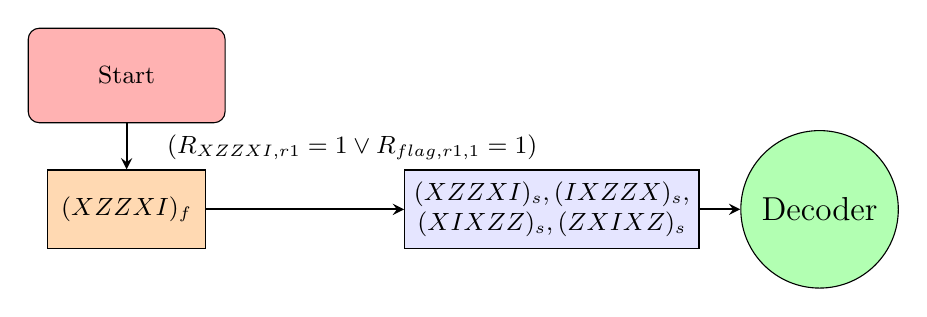
\begin{tikzpicture}[node distance=1.2cm, font=\mid] 
        
        % --- 1. Define Styles (Upgraded to \Large, slightly reduced minimum widths) ---
        \tikzstyle{startstop} = [rectangle, rounded corners, minimum width=2.5cm, minimum height=1.2cm, text centered, draw=black, fill=red!30, font=\small]
        \tikzstyle{raw_syn} = [rectangle, minimum width=2cm, minimum height=1cm, text centered, align=center, draw=black, fill=blue!10, font=\small]
        \tikzstyle{flag_syn} = [rectangle, minimum width=2cm, minimum height=1cm, text centered, align=center, draw=black, fill=orange!30, font=\small]
        \tikzstyle{decode} = [circle, minimum width=2cm, minimum height=1cm, text centered, align=center, draw=black, fill=green!30, font=\large]
        \tikzstyle{arrow} = [thick,->,>=stealth, font=\small] % Arrow math slightly smaller so it fits the lines

        % --- 2. Place Nodes ---
        \node (start) [startstop] {Start};
        
        % --- Step 1 ---
        \node (pro1) [flag_syn, below of=start, yshift=-0.5cm] {$(XZZXI)_{f}$};
        % Tightened xshift to 4.2cm so the diagram fits on the page naturally
        \node (pro2b) [raw_syn, right of=pro1, xshift=4.2cm] {$(XZZXI)_s, (IXZZX)_s,$\\$(XIXZZ)_s,(ZXIXZ)_s $};
        \node (decode1) [decode, right of=pro2b, xshift=2.2cm] {Decoder};
        
        

        % --- 3. Draw Arrows ---
        \draw [arrow] (start) -- (pro1);
        \draw [arrow] (pro1) -- node[above,xshift= 0.6cm, yshift = 0.5cm] {$(R_{XZZXI,r1}=1 \vee R_{flag,r1,1}=1)$} (pro2b);

        \draw [arrow] (pro2b) -- (decode1);


    \end{tikzpicture}
    \end{adjustbox}
    \caption{path 1 of Fig.~\ref{fig:flowchart}}
    \label{fig:flowchart_path_1}
\end{figure}






\paragraph{\textbf{Example}}
Fig.~\ref{fig:flowchart_path_1} illustrates the first path of the flagged syndrome extraction protocol for the $[[5, 1, 3]]$ QECC Fig.~\ref{fig:flowchart}, consisting of five distinct paths. For the first path, the protocol executes a flagged stabilizer extraction $(XZZXI)_f$ in the first round. If the measurement outcome satisfies the condition $(R_{XZZXI,r1,1} = 1 \lor R_{flag,r1,1} = 1)$, it proceeds to the second(last) round of syndrome extraction circuit of the stabilizers $$\big( (XZZXI)_s, (IXZZX)_s, (XIXZZ)_s, (ZXIXZ)_s \big)$$.

This path requires five data qubits, one ancilla qubit, and one flag qubit in the first round, followed by four additional ancilla qubits in the second round. The Pauli representation of the state of all qubits is:
\begin{equation}
Q =  Q_{d_1} \dots Q_{d_5} \ Q_{ancX, r1, 1} Q_{flagZ, r1, 1} \ Q_{ancX, r2, 1} \dots Q_{ancX, r2, 4} 
\end{equation}
where the subscripts $r1$ and $r2$ denote usage in Round 1 or Round 2, respectively. All qubits are initialized to $(0,0)$, and symbolic errors are injected by the variables $e^{p}_{c/t,x/z} $ after each gate operation.

Fig.~\ref{fig:step3_example_a} and \ref{fig:step3_example_b} depict the execution of the syndrome extraction circuit in Round 1 and Round 2. From this execution, we derive $\mathrm{Constraint_\mathrm{fault}}$. Based on the measurement outcomes $R_{XZZXI, r1,1}$ and $R_{flag,r1,1}$, we establish the path constraint:
\begin{equation}
\mathrm{Constraint}_\mathrm{path}: \Phi  = (R_{XZZXI, r1,1} = 1 \lor R_{flag,r1,1} = 1)
\end{equation}

The syndrome of the last round is collected as follows:
\begin{equation}
\begin{aligned}
    \mathrm{Syn}_{\mathrm{last}, XZZXI} &= R_{XZZXI, r2,1} \\
    \mathrm{Syn}_{\mathrm{last}, IXZZX} &= R_{IXZZX, r2,2} \\
    \mathrm{Syn}_{\mathrm{last}, XIXZZ} &= R_{XIXZZ, r2,3} \\
    \mathrm{Syn}_{\mathrm{last}, ZXIXZ} &= R_{ZXIXZ, r2,4} 
\end{aligned}
\end{equation}

Using the remaining data Pauli error after the second(last) round on the qubits $$E = Q^{last}_{d_1} Q^{last}_{d_2} Q^{last}_{d_3} Q^{last}_{d_4} Q^{last}_{d_5}$$, we can calculate the Boolean commutation relation $S_{P_k,E}$ and construct $\mathrm{Constraint}_{\mathrm{last\_syndrome}}$. The generalized syndrome $mgs$ is the set of all measurement outcomes from both rounds:
\begin{equation}
mgs = \{ R_{XZZXI, r1,1}, \ R_{flag,r1,1}, \ R_{XZZXI, r2,1}, \ R_{IXZZX, r2,2}, \ R_{XIXZZ, r2,3}, \ R_{ZXIXZ, r2,4}\}
\end{equation}

By duplicating the variables, we generate $\mathrm{Constraint}_{\mathrm{syn\_gen}}$ and all the $(1), (2)$ versions of the constraints derived previously. Let $E^{(1)} = Q^{last,(1)}_{d_1} \dots  Q^{last,(1)}_{d_5}$ and $E^{(2)} =  Q^{last,(2)}_{d_1} \dots  Q^{last,(2)}_{d_5}$. Given that the generators of the $[[5,1,3]]$ code are $G_1 = XZZXI$, $G_2 = IXZZX$, $G_3=XIXZZ$, and $G_4 = ZXIXZ$, we formulate $\mathrm{Constraint}_{\mathrm{non-degenerate}}$. By all the constraints:
\begin{equation}
\begin{aligned}
\mathrm{Constraint}_{\mathrm{total}} &= \mathrm{Constraint}_{\mathrm{path}}^{(1)} \land \mathrm{Constraint}_{\mathrm{fault}}^{(1)} \land \mathrm{Constraint}_{\mathrm{last\_syndrome}}^{(1)} \\
&\quad \land \mathrm{Constraint}_{\mathrm{path}}^{(2)} \land \mathrm{Constraint}_{\mathrm{fault}}^{(2)} \land \mathrm{Constraint}_{\mathrm{last\_syndrome}}^{(2)} \\
&\quad \land \mathrm{Constraint}_{\mathrm{syn\_gen}} \land \mathrm{Constraint}_{\mathrm{non-degenerate}} 
\end{aligned}
\end{equation}
we can use SAT solver to verify. The result is \texttt{unsat} which means that there cannot be two different fault events that resulting with same two generalized syndromes but the errors are non-degnerate. 
 
\begin{figure}[h]
    \centering
    % --- Subfigure (a): Round 1 ---
    \begin{subfigure}{0.8\linewidth}
        \centering
        \scalebox{0.9}{ % Adjust this value (0.6) to scale smaller or larger
        \begin{quantikz}[row sep={0.6cm,between origins}, column sep=0.4cm, font=\large]
            % Data Qubits
            \lstick{$Q_{d_1} = (0,0)$} & & \gate[7]{(XZZXI)_f} & \rstick{$Q'_{d_1} = (Q'_{d_1,x},Q'_{d_1,z})$} \\
            \lstick{$Q_{d_2} = (0,0)$} & & & \rstick{$Q'_{d_2} = (Q'_{d_2,x},Q'_{d_2,z})$} \\
            \lstick{$Q_{d_3} = (0,0)$} & & & \rstick{$Q'_{d_3} = (Q'_{d_3,x},Q'_{d_3,z})$} \\
            \lstick{$Q_{d_4} = (0,0)$} & & & \rstick{$Q'_{d_4} = (Q'_{d_4,x},Q'_{d_4,z})$} \\
            \lstick{$Q_{d_5} = (0,0)$} & & & \rstick{$Q'_{d_5} = (Q'_{d_5,x},Q'_{d_5,z})$} \\
            % Measurement Qubits
            \lstick{$Q_{ancX, r1,1} = (0, 0)$}   & & & \rstick{$R_{XZZXI, r1,1}$} \\
            \lstick{$Q_{flagZ, r1, 1} = (0, 0)$} & & & \rstick{$R_{flag,r1,1}$}
        \end{quantikz}
        }
        \caption{First round: Flagged syndrome extraction.}
        \label{fig:step3_example_a}
    \end{subfigure}
    \hfill
    % --- Subfigure (b): Round 2 ---
    \begin{subfigure}{0.8\linewidth}
        \centering
        \scalebox{0.9}{ % Adjust this value (0.6) to scale smaller or larger
        \begin{quantikz}[row sep={0.6cm,between origins}, column sep=0.4cm, font=\large]
            % Inputs from Round 1
            \lstick{$Q'_{d_1}$} & & \gate[9]{\begin{array}{c} (XZZXI)_s \\ (IXZZX)_s \\ (XIXZZ)_s \\ (ZXIXZ)_s \end{array}} & \rstick{$Q^{\mathrm{last}}_{d_1} = (Q^{\mathrm{last}}_{d_1,x},Q^{\mathrm{last}}_{d_1,z})$} \\
            \lstick{$Q'_{d_2}$} & & & \rstick{$Q^{\mathrm{last}}_{d_2} = (Q^{\mathrm{last}}_{d_2,x},Q^{\mathrm{last}}_{d_2,z})$} \\
            \lstick{$Q'_{d_3}$} & & & \rstick{$Q^{\mathrm{last}}_{d_3} = (Q^{\mathrm{last}}_{d_3,x},Q^{\mathrm{last}}_{d_3,z})$} \\
            \lstick{$Q'_{d_4}$} & & & \rstick{$Q^{\mathrm{last}}_{d_4} = (Q^{\mathrm{last}}_{d_4,x},Q^{\mathrm{last}}_{d_4,z})$} \\
            \lstick{$Q'_{d_5}$} & & & \rstick{$Q^{\mathrm{last}}_{d_5} = (Q^{\mathrm{last}}_{d_5,x},Q^{\mathrm{last}}_{d_5,z})$} \\
            % Ancilla Outcomes
            \lstick{$Q_{ancX, r2,1} = (0, 0)$} & & & \rstick{$R_{XZZXI, r2,1}$} \\
            \lstick{$Q_{ancX, r2,2} = (0, 0)$} & & & \rstick{$R_{IXZZX, r2,2}$} \\
            \lstick{$Q_{ancX, r2,3} = (0, 0)$} & & & \rstick{$R_{XIXZZ, r2,3}$} \\
            \lstick{$Q_{ancX, r2,4} = (0, 0)$} & & & \rstick{$R_{ZXIXZ, r2,4}$}
        \end{quantikz}
        }
        \caption{Second round: Final syndrome extraction.}
        \label{fig:step3_example_b}
    \end{subfigure}

    \caption{Symbolic execution example for Step 3.}
    \label{fig:step3_example}
\end{figure}


\fi


\section{Related Work}

Recent works have made significant progress in verifying quantum error correction circuits using SAT solvers. For example, Chen et al.~\cite{chen2025verifying} employ symbolic execution to check if injected faults in quantum gadgets violate fault-tolerance conditions. Similarly, Huang et al.~\cite{10.1145/3729293} introduce Veri-QEC, a formal verification framework that translates Pauli errors into classical assertions solved by SAT solvers. 

However, applying these general methods to flagged syndrome extraction circuits creates a major bottleneck if an explicit decoder is not provided. In these frameworks, two distinct faults might produce the exact same syndrome. Without a predefined decoder to resolve this ambiguity, their tools cannot determine whether the post-recovery state will actually cause a logical error. Furthermore, their assertions struggle when an error propagates to a weight strictly greater than $t$---a scenario that naturally occurs in flagged protocols.

Our work bypasses these limitations by adopting a specialized approach. By focusing strictly on flagged syndrome extraction protocols, we completely eliminate the need for a decoder during the verification process. Instead of directly evaluating standard fault-tolerance conditions, we verify a necessary and sufficient property: \emph{distinguishability}. If a flagged protocol passes our distinguishability check, we can mathematically guarantee the existence of a valid look-up-table (LUT) decoder for it. Beyond these theoretical guarantees, our approach demonstrates clear practical utility; by applying our method, we successfully identified previously unknown design flaws in published flagged syndrome extraction protocols.

\section{Results}
\begin{table}[htbp]
\centering
\begin{tabular}{lccccc}
\toprule
Code & Circuit Optimization & Protocol & Step 1 & Step 2 & Step 3 \\
\midrule
$[[5,1,3]]$  & $[1,1,1,1]^{T}$           & [LL25] $d=3$ & Pass & Pass & Pass \\
$[[5,1,3]]$  & $[2,2]^{T}$               & [LL25] $d=3$ & Pass & Pass & Fail \\
$[[5,1,3]]$  & $[2,2]$                   & [LL25] $d=3$ & Pass & Pass & Fail \\
$[[19,1,5]]$ & $\mathbf{[1]}^T$          & [LL25] $d=5$ & Pass & Pass & Pass \\
$[[19,1,5]]$ & $[2,2,2,1,1,1]^{T}$       & [LL25] $d=5$ & Pass & Fail & Pass \\
$[[19,1,5]]$ & Parallel flagged          & [Du24] $d=5$ & Pass & Fail & Pass \\
$[[7,1,3]]$  & Sequential                & [CB18] $d=3$ & Pass & Pass & Pass \\

$[[25,1,5]]$ & Sequential                & [CB18] $d=5$ & Pass & Pass & Pass \\
$[[17,1,5]]$ & Sequential                & [CB18] $d=5$ & Pass & Pass & Pass \\
$[[5,1,3]]$  & Low-depth                 & [Bha23]      & Pass & Fail & Fail \\
$[[7,1,3]]$  & Low-depth                 & [Bha23]      & Pass & Pass & Pass \\
\bottomrule
\end{tabular}
\caption{Verification results of flagged syndrome extraction protocols. Protocols are sourced from \cite{Liou25} [LL25], \cite{Chamberland18} [CB18], \cite{Du24} [Du24], and \cite{low-depth} [Bha23]. Columns 1--3 describe the QECC, circuit optimization, and protocol strategy, respectively. Columns 4--6 report the verification results for Steps 1 through 3 of our framework.}\label{tab:experiment-results}
\end{table}

Our experiments were conducted on a MacBook Pro with an M4 Pro chip and 48GB of RAM. We implemented our verification framework using Z3py to encode the constraints, which were subsequently transformed into DIMACS format for the CryptoMiniSat solver. CryptoMiniSat was chosen for its highly optimized performance on formulas containing massive XOR clauses; all tasks were run without a timeout. 

An interesting finding in Table~\ref{tab:experiment-results} is that the $[[19,1,5]]$ protocols from \cite{Liou25} and \cite{Du24} failed Step 2 but passed Step 3. This means that while some individual circuits fail to raise a flag for high-weight errors, the overall protocol remains safe. As noted in \cite{Liou25, Du24}, a local failure in a single flagged extraction circuit does not necessarily break the distinguishability of the entire protocol. Our results formally confirm this: the multi-round structure of these protocols ensures that even if a flag is missed in one round, the final syndrome remains unique and the errors can still be distinguished.


By applying our tool to existing flagged syndrome extraction protocols, we identified several design flaws that violate the stated fault-tolerance properties. We highlight two representative flaws discovered by our verification, both of which were found in protocols based on the $[[5,1,3]]$ stabilizer code. 

\paragraph{Example 1 (\cite{Liou25} protocol with the $[2,2]^T$ circuit).}
Fig.~\ref{fig:[[5,1,3]]-[2,2]^T-fail} shows a counterexample for the $[[5,1,3]]$
code using the $[2,2]^T$ syndrome-extraction circuit together with the Liou
($d=3$) protocol. The two subfigures correspond to the first round of the
protocol under two different single-gate faults. In both cases, the fault (red)
induces a Pauli error that propagates through the circuit (blue). Although the
resulting Pauli operators on the ancilla and flag qubits differ, the measurement
outcomes are identical: since the ancilla is prepared and measured in the $X$
basis, both $Y$ and $Z$ errors have the same effect on the measurement result.

Because the fault occurs in the first round, the second (last) round (not shown) is
fault-free. The two resulting data-qubit errors, $IIZIX$ and $IZIIZ$, produce the
same syndrome in the last round. Therefore, the entire generalized
syndrome (including syndrome and flag outcomes across rounds) is identical in
the two executions. However, the two data-qubit errors are non-degenerate, which
violates Proposition~\ref{prop:flagged_syndrome_extraction_protocol}.

Using our verification framework, we can rapidly evaluate new circuit designs. As a demonstration, Fig.~\ref{fig:fixed_extraction_circuit} presents a corrected flagged syndrome extraction circuit that maintains the original optimization goals while strictly satisfying our verification conditions.





\begin{figure}[h]
\centering

\begin{subfigure}{0.2\linewidth} 
\hspace*{-5.5cm}
\centering
\scalebox{0.7}{
\begin{quantikz}[column sep =0.3cm]
\lstick{$Q_{d_1}$}   & \ctrl{7}   & \qw        & \qw        & \qw        & \qw      & \qw      & \qw        & \qw      & \qw        & \qw      & \ctrl{8}   & \qw                                                                                                                                                       & \qw                        & \qw        & \qw        & \targ{}    & \qw        & \qw      & \qw      & \targ{}    & \qw      & \qw      & \qw        & \qw        & \qw      & \qw            & \qw            \\
\lstick{$Q_{d_2}$}   & \qw        & \ctrl{4}   & \qw        & \qw        & \qw      & \qw      & \ctrl{6}   & \qw      & \qw        & \qw      & \qw        & \qw                                                                                                                                                       & \qw                        & \qw        & \qw        & \qw        & \targ{}    & \qw      & \qw      & \qw        & \qw      & \qw      & \qw        & \qw        & \qw      & \qw            & \qw             \\
\lstick{$Q_{d_3}$}   & \qw        & \qw        & \targ{}    & \qw        & \qw      & \qw      & \qw        & \qw      & \ctrl{3}   & \qw      & \qw        & \targ{} \gategroup[6,steps=1,style={dashed,rounded corners,fill=red!20},background,label style={label position=below}]{{\sc Fault}} & \gate[style={draw=red}]{Z} & \qw        & \qw        & \qw        & \qw        & \qw      & \qw      & \qw        & \qw      & \qw      & \qw        & \qw        & \qw      & \gate[style={draw=blue}]{Z} & \qw\\
\lstick{$Q_{d_4}$}   & \qw        & \qw        & \qw        & \targ{}    & \qw      & \qw      & \qw        & \qw      & \qw        & \qw      & \qw        & \qw                                                                                                                                                       & \qw                        & \targ{}    & \qw        & \qw        & \qw        & \qw      & \qw      & \qw        & \qw      & \qw      & \qw        & \ctrl{3}   & \qw      & \qw             & \qw           \\
\lstick{$Q_{d_5}$}   & \qw        & \qw        & \qw        & \qw        & \qw      & \qw      & \qw        & \qw      & \qw        & \qw      & \qw        & \qw                                                                                                                                                       & \qw                        & \qw        & \ctrl{2}   & \qw        & \qw        & \qw      & \qw      & \qw        & \qw      & \qw      & \targ{}    & \qw        & \ctrl{4} & \gate[style={draw=blue}]{X} & \qw \\
\lstick{$Q_{ancX,1}$}  & \qw        & \control{} & \qw        & \qw        & \ctrl{4} & \qw      & \qw        & \qw      & \control{} & \qw      & \qw        & \qw                                                                                                                                                       & \qw                        & \ctrl{-2}  & \qw        & \qw        & \qw        & \ctrl{4} & \qw      & \ctrl{-5}  & \qw      & \qw      & \qw        & \qw        & \qw      & \qw             &\meter{X}         \\
\lstick{$Q_{ancX,2}$}  & \qw        & \qw        & \ctrl{-4}  & \qw        & \qw      & \qw      & \qw        & \qw      & \qw        & \ctrl{3} & \qw        & \qw                                                                                                                                                       & \qw                        & \qw        & \control{} & \ctrl{-6}  & \qw        & \qw      & \qw      & \qw        & \ctrl{3} & \qw      & \qw        & \control{} & \qw      & \qw             &\meter{X}       \\
\lstick{$Q_{ancX,3}$}  & \control{} & \qw        & \qw        & \qw        & \qw      & \ctrl{3} & \control{} & \qw      & \qw        & \qw      & \qw        & \ctrl{-5}                                                                                                                                                 & \gate[style={draw=red}]{X} & \qw        & \qw        & \qw        & \qw        & \qw      & \ctrl{3} & \qw        & \qw      & \qw      & \ctrl{-3}  & \qw        & \qw      & \gate[style={draw=blue}]{X}  &\meter{X}\\
\lstick{$Q_{ancX,4}$}  & \qw        & \qw        & \qw        & \ctrl{-5}  & \qw      & \qw      & \qw        & \ctrl{2} & \qw        & \qw      & \control{} & \qw                                                                                                                                                       & \qw                        & \qw        & \qw        & \qw        & \ctrl{-7}  & \qw      & \qw      & \qw        & \qw      & \ctrl{2} & \qw        & \qw        & \control{}& \gate[style={draw=blue}]{Z}  &\meter{X}\\
\lstick{$Q_{flagZ,1}$} & \qw        & \qw        & \qw        & \qw        & \targ{}  & \qw      & \qw        & \qw      & \qw        & \targ{}  & \qw        & \qw                                                                                                                                                       & \qw                        & \qw        & \qw        & \qw        & \qw        & \targ{}  & \qw      & \qw        & \targ{}  & \qw      & \qw        & \qw        & \qw      & \qw      &\meter{Z}                  \\
\lstick{$Q_{flagZ,2}$} & \qw        & \qw        & \qw        & \qw        & \qw      & \targ{}  & \qw        & \targ{}  & \qw        & \qw      & \qw        & \qw                                                                                                                                                       & \qw                        & \qw        & \qw        & \qw        & \qw        & \qw      & \targ{}  & \qw        & \qw      & \targ{}  & \qw        & \qw        & \qw      & \gate[style={draw=blue}]{X} &\meter{Z}
\end{quantikz}
}
\caption{}
\label{fig:left-circuit-22T}
\end{subfigure}

\vfill

\begin{subfigure}{0.2\linewidth}
\hspace*{-5.5cm}
\scalebox{0.7}{
\begin{quantikz}[column sep =0.3cm]
\lstick{$Q_{d_1}$}     & \ctrl{7}   & \qw        & \qw        & \qw        & \qw      & \qw      & \qw        & \qw      & \qw        & \qw      & \ctrl{8}   & \qw        & \qw        & \qw        & \targ{}    & \qw    & \qw    & \qw      & \qw      & \targ{}    & \qw      & \qw      & \qw        & \qw        & \qw   & \qw   & \qw        \\
\lstick{$Q_{d_2}$}     & \qw        & \ctrl{4}   & \qw        & \qw        & \qw      & \qw      & \ctrl{6}   & \qw      & \qw        & \qw      & \qw        & \qw        & \qw        & \qw        & \qw       & \targ{}\gategroup[8,steps=1,style={dashed,rounded corners,fill=red!20},background,label style={label position=below}]{{\sc Fault}} & \gate[style = {draw=red}]{Z}   & \qw      & \qw      & \qw        & \qw      & \qw      & \qw        & \qw        & \qw   & \gate[style = {draw=blue}]{Z} & \qw  \\
\lstick{$Q_{d_3}$}     & \qw        & \qw        & \targ{}    & \qw        & \qw      & \qw      & \qw        & \qw      & \ctrl{3}   & \qw      & \qw        & \targ{}    & \qw        & \qw        & \qw        & \qw     & \qw   & \qw      & \qw      & \qw        & \qw      & \qw      & \qw        & \qw        & \qw   & \qw & \qw     \\
\lstick{$Q_{d_4}$}     & \qw        & \qw        & \qw        & \targ{}    & \qw      & \qw      & \qw        & \qw      & \qw        & \qw      & \qw        & \qw        & \targ{}    & \qw        & \qw        & \qw     & \qw   & \qw      & \qw      & \qw        & \qw      & \qw      & \qw        & \ctrl{3}   & \qw   & \qw  & \qw    \\
\lstick{$Q_{d_5}$}     & \qw        & \qw        & \qw        & \qw        & \qw      & \qw      & \qw        & \qw      & \qw        & \qw      & \qw        & \qw        & \qw        & \ctrl{2}   & \qw        & \qw    & \qw    & \qw      & \qw      & \qw        & \qw      & \qw      & \targ{}    & \qw        & \ctrl{4}  &\gate[style = {draw=blue}]{Z}  & \qw    \\
\lstick{$Q_{ancX,1}$}  & \qw        & \control{} & \qw        & \qw        & \ctrl{4} & \qw      & \qw        & \qw      & \control{} & \qw      & \qw        & \qw        & \ctrl{-2}  & \qw        & \qw        & \qw      & \qw  & \ctrl{4} & \qw      & \ctrl{-5}  & \qw      & \qw      & \qw        & \qw        & \qw        & \qw  &\meter{X} \\
\lstick{$Q_{ancX,2}$}  & \qw        & \qw        & \ctrl{-4}  & \qw        & \qw      & \qw      & \qw        & \qw      & \qw        & \ctrl{3} & \qw        & \qw        & \qw        & \control{} & \ctrl{-6}  & \qw      & \qw  & \qw      & \qw      & \qw        & \ctrl{3} & \qw      & \qw        & \control{} & \qw        & \qw &\meter{X}  \\
\lstick{$Q_{ancX,3}$}  & \control{} & \qw        & \qw        & \qw        & \qw      & \ctrl{3} & \control{} & \qw      & \qw        & \qw      & \qw        & \ctrl{-5}  & \qw        & \qw        & \qw        & \qw      & \qw  & \qw      & \ctrl{3} & \qw        & \qw      & \qw      & \ctrl{-3}  & \qw        & \qw       & \qw  &\meter{X}  \\
\lstick{$Q_{ancX,4}$}  & \qw        & \qw        & \qw        & \ctrl{-5}  & \qw      & \qw      & \qw        & \ctrl{2} & \qw        & \qw      & \control{} & \qw        & \qw        & \qw        & \qw        & \ctrl{-7}&\gate[style = {draw=red}]{Y}  & \qw      & \qw      & \qw        & \qw      & \ctrl{2} & \qw        & \qw        & \control{} & \gate[style = {draw=blue}]{Y} &\meter{X}\\
\lstick{$Q_{flagZ,1}$} & \qw        & \qw        & \qw        & \qw        & \targ{}  & \qw      & \qw        & \qw      & \qw        & \targ{}  & \qw        & \qw        & \qw        & \qw        & \qw        & \qw      & \qw  & \targ{}  & \qw      & \qw        & \targ{}  & \qw      & \qw        & \qw        & \qw      & \qw  &\meter{Z}  \\
\lstick{$Q_{flagZ,2}$} & \qw        & \qw        & \qw        & \qw        & \qw      & \targ{}  & \qw        & \targ{}  & \qw        & \qw      & \qw        & \qw        & \qw        & \qw        & \qw        & \qw      & \qw  & \qw      & \targ{}  & \qw        & \qw      & \targ{}  & \qw        & \qw        & \qw      & \gate[style = {draw=blue}]{X} &\meter{Z}
\end{quantikz}
}
\caption{}
\label{fig:right-circuit-22T}
\end{subfigure}

\caption{Counterexample showing indistinguishable errors arising from different faults in the $[2,2]^T$ circuit}
\label{fig:[[5,1,3]]-[2,2]^T-fail}
\end{figure}

\begin{figure}[h]
\centering
\begin{adjustbox}{max width= 0.9\textwidth}
\begin{quantikz}[row sep=0.5cm, column sep=0.3cm]
\lstick{$Q_{d_1}$}   & \qw      & \targ{}   & \qw       & \qw       & \qw       & \qw      & \qw      & \qw      & \qw      & \qw        & \qw        & \qw        & \qw        & \ctrl{8}   & \qw        & \qw        & \qw        & \qw      & \qw      & \qw      & \qw      & \qw       & \qw       & \targ{}   & \qw & \qw \\
\lstick{$Q_{d_2}$}   & \qw      & \qw       & \targ{}   & \qw       & \qw       & \qw      & \qw       & \qw      & \qw      & \ctrl{4}   & \qw        & \qw        & \qw        & \qw        & \qw        & \ctrl{6}   & \qw        & \qw      & \qw      & \qw      & \qw      & \qw       & \qw       & \qw       & \targ{}  & \qw\\
\lstick{$Q_{d_3}$}   & \qw      & \qw       & \qw       & \targ{}   & \qw       & \qw      & \qw      & \qw      & \qw      & \qw        & \qw        & \ctrl{3}   & \qw        & \qw        & \ctrl{6}   & \qw        & \qw        & \qw      & \qw      & \qw      & \qw      & \qw       & \qw       & \qw       & \qw & \qw\\
\lstick{$Q_{d_4}$}   & \qw      & \qw       & \qw       & \qw       & \targ{}   & \qw      & \qw      & \qw      & \qw      & \qw        & \ctrl{4}   & \qw        & \qw        & \qw        & \qw        & \qw        & \ctrl{3}   & \qw      & \qw      & \qw      & \qw      & \targ{}   & \qw       & \qw       & \qw & \qw\\
\lstick{$Q_{d_5}$}   & \qw      & \qw       & \qw       & \qw       & \qw       & \qw      & \qw      & \qw      & \qw      & \qw        & \qw        & \qw        & \ctrl{2}   & \qw        & \qw        & \qw        & \qw        & \qw      & \qw      & \qw      & \qw      & \qw       & \targ{}   & \qw       & \qw & \qw\\
\lstick{$Q_{ancX,1}$}  & \gate{H} & \ctrl{-5} & \qw       & \qw       & \qw       & \ctrl{5} & \qw      & \qw      & \qw      & \control{} & \qw        & \control{} & \qw        & \qw        & \qw        & \qw        & \qw        & \ctrl{5} & \qw      & \qw      & \qw      & \ctrl{-2} & \qw       & \qw       & \qw &\meter{X}\\
\lstick{$Q_{ancX,2}$}  & \gate{H} & \qw       & \ctrl{-5} & \qw       & \qw       & \qw      & \qw      & \ctrl{4} & \qw      & \qw        & \qw        & \qw        & \control{} & \qw        & \qw        & \qw        & \control{} & \qw      & \qw      & \ctrl{4} & \qw      & \qw       & \ctrl{-2} & \qw       & \qw &\meter{X}\\
\lstick{$Q_{ancX,3}$}  & \gate{H} & \qw       & \qw       & \ctrl{-5} & \qw       & \qw      & \ctrl{2} & \qw      & \qw      & \qw        & \control{} & \qw        & \qw        & \qw        & \qw        & \control{} & \qw        & \qw      & \ctrl{2} & \qw      & \qw      & \qw       & \qw       & \ctrl{-7} & \qw&\meter{X} \\
\lstick{$Q_{ancX,4}$}  & \gate{H} & \qw       & \qw       & \qw       & \ctrl{-5} & \qw      & \qw      & \qw      & \ctrl{1} & \qw        & \qw        & \qw        & \qw        & \control{} & \control{} & \qw        & \qw        & \qw      & \qw      & \qw      & \ctrl{1} & \qw       & \qw       & \qw       & \ctrl{-7} &\meter{X}\\
\lstick{$Q_{flagZ,1}$} & \qw      & \qw       & \qw       & \qw       & \qw       & \qw      & \targ{}  & \qw      & \targ{}  & \qw        & \qw        & \qw        & \qw        & \qw        & \qw        & \qw        & \qw        & \qw      & \targ{}  & \qw      & \targ{}  & \qw       & \qw       & \qw       & \qw &\meter{Z}\\
\lstick{$Q_{flagZ,2}$} & \qw      & \qw       & \qw       & \qw       & \qw       & \targ{}  & \qw      & \targ{}  & \qw      & \qw        & \qw        & \qw        & \qw        & \qw        & \qw        & \qw        & \qw        & \targ{}  & \qw      & \targ{}  & \qw      & \qw       & \qw       & \qw       & \qw &\meter{Z}
\end{quantikz}
\end{adjustbox}
\caption{The fixed circuit of example 1}
\label{fig:fixed_extraction_circuit}
\end{figure}


\paragraph{Example 2 (Low-depth adaptive protocol \cite{low-depth}).}
We also found a counterexample in the low-depth adaptive protocol of
\cite{low-depth}. Fig.~\ref{fig:[[5,1,3]]-low-depth-fault} shows two executions in
which a single fault occurs in the first-round measurement of $XZZXI$ using a
flag qubit. In one case, the fault on the first $\mathrm{CZ}$ gate induces an
$XY$ error; in the other case, a fault on the second $\mathrm{CZ}$ gate induces a
$YY$ error. In both executions, the syndrome bit and the flag outcome are
identical. The protocol then proceeds to measure $XZZXI$, $YXXYI$, and $XIXZZ$
without flags, yielding identical measurement outcomes across the two runs.
Nevertheless, the resulting data-qubit errors are $IIYXI$ and $IXZXI$, which are
non-degenerate. Hence, the protocol violates
Proposition~\ref{prop:flagged_syndrome_extraction_protocol}.

Designing flagged syndrome extraction circuits is highly error-prone; even for small codes such as the $[[5,1,3]]$ code, pursuing different optimization goals can introduce faults that are difficult to identify manually. To address this, our verification framework enables rapid prototyping and iteration, substantially reducing the time required to develop and validate new extraction protocols for diverse quantum codes.
\begin{figure}[h]
\centering

\begin{subfigure}{0.48\linewidth}
\centering
\scalebox{0.7}{
\begin{quantikz}[row sep={1cm,between origins}, column sep=0.45cm]
\lstick{$Q_{d_1}$}   & \targ{}   & \qw      & \qw        & \qw        & \qw                        & \qw      & \qw        & \qw & \qw                         & \qw\\
\lstick{$Q_{d_2}$}   & \qw       & \qw      & \control{} & \qw        & \qw                        & \qw      & \qw        & \qw & \qw                         & \qw\\
\lstick{$Q_{d_3}$}   & \qw       & \qw      & \qw        & \control{}\gategroup[4,steps=1,style={dashed,rounded corners,fill=red!20},background,label style={label position=above}]{{\sc Fault}} & \gate[style={draw=red}]{Y} & \qw      & \qw        & \qw & \gate[style={draw=blue}]{Y} & \qw\\
\lstick{$Q_{d_4}$}   & \qw       & \qw      & \qw        & \qw        & \qw                        & \qw      & \targ{}    & \qw & \gate[style={draw=blue}]{X} & \qw\\
\lstick{$Q_{d_5}$}   & \qw       & \qw      & \qw        & \qw        & \qw                        & \qw      & \qw        & \qw & \qw                         & \qw\\
\lstick{$Q_{ancX}$}  & \ctrl{-5} & \ctrl{1} & \ctrl{-4}  & \ctrl{-3}  & \gate[style={draw=red}]{Y} & \ctrl{1} & \ctrl{-2}  & \qw & \gate[style={draw=blue}]{Y} & \meter{X}\\
\lstick{$Q_{flagZ}$} & \qw       & \targ{}  & \qw        & \qw        & \qw                        & \targ{}  & \qw        & \qw & \gate[style={draw=blue}]{X} & \meter{Z}
\end{quantikz}
}
\caption{}
\label{fig:left-circuit-ld}
\end{subfigure}%
\hfill
\begin{subfigure}{0.48\linewidth}
\centering
\scalebox{0.7}{
\begin{quantikz}[row sep={1cm,between origins}, column sep=0.45cm]
\lstick{$Q_{d_1}$}   & \targ{}   & \qw      & \qw   & \qw      & \qw      & \qw      & \qw      & \qw & \qw                         & \qw \\
\lstick{$Q_{d_2}$}   & \qw       & \qw      & \control{} \gategroup[5,steps=1,style={dashed,rounded corners,fill=red!20},background,label style={label position=above}]{{\sc Fault}} & \gate[style={draw=red}]{X}   & \qw      & \qw      & \qw      & \qw & \gate[style={draw=blue}]{X}  & \qw\\
\lstick{$Q_{d_3}$}   & \qw       & \qw      & \qw     & \qw    & \control{}  & \qw      & \qw      & \qw & \gate[style={draw=blue}]{Z}  & \qw\\
\lstick{$Q_{d_4}$}   & \qw       & \qw      & \qw    & \qw     & \qw      & \qw      & \targ{}  & \qw & \gate[style={draw=blue}]{X}  & \qw \\
\lstick{$Q_{d_5}$}   & \qw       & \qw      & \qw    & \qw     & \qw      & \qw      & \qw      & \qw & \qw                         & \qw \\
\lstick{$Q_{ancX}$}  & \ctrl{-5} & \ctrl{1} & \ctrl{-4}&\gate[style={draw=red}]{Y}   & \ctrl{-3} & \ctrl{1} & \ctrl{-2} & \qw & \gate[style={draw=blue}]{Y} & \meter{X}\\
\lstick{$Q_{flagZ}$} & \qw       & \targ{}  & \qw       & \qw      & \targ{}  & \qw      & \qw      & \qw & \gate[style={draw=blue}]{X} & \meter{Z}
\end{quantikz}
}
\caption{}
\label{fig:right-circuit-ld}
\end{subfigure}

\caption{Counterexample showing identical syndrome and flag outcomes in the Exmaple 2}
\label{fig:[[5,1,3]]-low-depth-fault}
\end{figure}



\section{Conclusion}
In this paper, we presented a formal verification framework for fault-tolerant flagged syndrome extraction protocols. Instead of directly verifying standard fault-tolerance definitions, we verified a necessary and sufficient distinguishability condition. While many protocols include manual proofs of fault tolerance, advanced optimizations---such as reduced circuit depth or flag qubit sharing---complicate gate ordering and error propagation, making manual verification prone to error. Our automated, SAT-based approach accelerates the design process by rapidly identifying whether a proposed circuit or protocol contains design flaws. 

In future work, we plan to extend our Pauli-tracking encoding to verify other fault-tolerant gadgets and broader quantum computing architectures, such as measurement-based quantum computation.


\section*{Data-Availability Statement}
The artifact consists of a python prototype used to support the results in the paper. The current version is complete but with restricted documentation. We intend to submit this artifact for Artifact Evaluation.




\clearpage
\bibliographystyle{ACM-Reference-Format} 
\bibliography{refs}

%\cy{Fig 7a  should be corrected: red ZZ do not propagate to the blue ZXXZX.  Should be red Z"X"}
\clearpage
\appendix

\section{Lemma Proof}
\begin{lemma}
For a QECC with a stabilizer group $\mathcal{S} = \langle g_1, \dots, g_{n-k} \rangle$ and logical operators $\mathcal{L} = \{\bar{X}_1, \dots, \bar{X}_k, \bar{Z}_1, \dots, \bar{Z}_k\}$, if a Pauli string $P$ commutes with all generators $g_i$ and all logical operators $\bar{X}_j, \bar{Z}_j$, then $P$ lies in the group $\mathcal{S}$ (up to an overall phase).
\end{lemma}

\begin{proof}
The codespace $\mathcal{C}$ stabilized by the group $\mathcal{S}$ is defined as:
\[
\mathcal{C} = \{\,|\psi\rangle : G|\psi\rangle = |\psi\rangle \ \forall G \in \mathcal{S}\,\}.
\]
Since $P$ commutes with every generator $G_i$, it commutes with all of $\mathcal{S}$. Hence, for any
$|\psi\rangle \in \mathcal{C}$ and any $G \in \mathcal{S}$,
\[
G(P|\psi\rangle) = P(G|\psi\rangle) = P|\psi\rangle,
\]
so $P$ maps $\mathcal{C}$ to itself.

Fix the logical computational basis $\{|z\rangle_L\}_{z\in\{0,1\}^k} \subset \mathcal{C}$
defined by
\[
\bar{Z}_j |z\rangle_L = (-1)^{z_j}|z\rangle_L \qquad (j=1,\dots,k).
\]
Because $P$ commutes with every $\bar{Z}_j$, it preserves each joint eigenspace of the
commuting family $\{\bar{Z}_j\}_{j=1}^k$. In particular, each $|z\rangle_L$ is an eigenvector of
$P$:
\[
P|z\rangle_L = \lambda_z |z\rangle_L
\]
for some phase $\lambda_z$ (indeed $\lambda_z \in \{\pm 1, \pm i\}$ since $P \in \mathcal{P}_n$).

Now use commutation with the logical $\bar{X}_j$. For any $j$ and any bitstring $z$,
\[
P(\bar{X}_j|z\rangle_L) = \bar{X}_j(P|z\rangle_L) = \lambda_z\,\bar{X}_j|z\rangle_L.
\]
Since $\bar{X}_j|z\rangle_L = |z\oplus e_j\rangle_L$, the left-hand side is also
\[
P|z\oplus e_j\rangle_L = \lambda_{z\oplus e_j}|z\oplus e_j\rangle_L,
\]
hence
\[
\lambda_{z\oplus e_j} = \lambda_z \qquad \forall z,\ \forall j.
\]
Because the bit flips $z \mapsto z\oplus e_j$ connect all bitstrings in $\{0,1\}^k$, it follows that
$\lambda_z$ is independent of $z$; write $\lambda_z=\lambda$ for all $z$. Therefore,
\[
P|\psi\rangle = \lambda |\psi\rangle \qquad \forall |\psi\rangle \in \mathcal{C},
\]
i.e., $P$ acts as a global phase on the entire codespace.

Equivalently, the induced logical operator of $P$ is trivial. Hence $P$ represents the
identity element in the quotient $C(\mathcal{S})/\mathcal{S}$, where $C(\mathcal{S})$ is the centralizer of $\mathcal{S}$. Thus, there exists an element $S' \in \mathcal{S}$ such that
$P = \lambda S'$. We conclude that $P \in \mathcal{S}$ up to an overall phase, as claimed.
\end{proof}


\end{document}